\documentclass[10pt]{beamer}
\usetheme{Copenhagen}
\usepackage[utf8]{inputenc}
\usepackage[french]{babel}
\usepackage[T1]{fontenc}
\usepackage{amsmath}
\usepackage{amsfonts}
\usepackage{amssymb}
\usepackage{graphicx}
\usepackage{relsize}
\usepackage{subcaption}
\usepackage{amsmath}
\usepackage{listings}
\usepackage{listingsutf8}
\usepackage{xcolor}
\usepackage{multicol}

\author{TRAN-THUONG Tien-Thinh [n°30903]}
\date{2021-2022}
\graphicspath{{Affiche/0-ReconnaissanceVocale/}{Affiche/1-Introduction/}{Affiche/2-Activation-Gradient/}{Affiche/4-XOR/}{Affiche/5-MNIST/}{Affiche/6-Mot/}{Affiche/7-Vocal/}}
\lstset{inputpath={Affiche/99-Code/}}
\newcommand{\norme}[1]{\| #1 \|}

\definecolor{codegreen}{rgb}{0,0.6,0}
\definecolor{codegray}{rgb}{0.5,0.5,0.5}
\definecolor{codepurple}{rgb}{0.58,0,0.82}
\definecolor{backcolour}{rgb}{0.95,0.95,0.92}
\lstdefinestyle{mystyle}{
    backgroundcolor=\color{backcolour},   
    commentstyle=\color{codegreen},
    keywordstyle=\color{magenta},
    numberstyle=\tiny\color{codegray},
    stringstyle=\color{codepurple},
    basicstyle=\ttfamily\footnotesize,
    breakatwhitespace=false,         
    breaklines=true,                 
    captionpos=b,                    
    keepspaces=true,                 
    numbers=left,                    
    numbersep=5pt,                  
    showspaces=false,                
    showstringspaces=false,
    showtabs=false,                  
    tabsize=1,
    xleftmargin=-5pt,
    xrightmargin=-10pt
}

\lstset{style=mystyle, inputencoding=utf8/latin1}
% \title{Reconnaissance vocale lors d’appel d’urgence grâce à un réseau de neurones}
\title{2021-2022 \hspace{15em} \insertframenumber\,/\,\inserttotalframenumber}
%  \setbeamertemplate{footline}[text line]{\parbox{\linewidth}{\vspace*{-8pt}\insertframenumber\,/\,\inserttotalframenumber Tra}



% \includeonly{sections/1-1, sections/1-2, sections/1-3, sections/1-4}
% \includeonly{sections/2-1, sections/2-2, sections/2-3, sections/2-4}
% \includeonly{sections/3-1, sections/3-2, sections/3-3, sections/3-4}
% \includeonly{sections/4-1, sections/4-2, sections/4-3, sections/4-4}
% Current section
\AtBeginSection[ ]
{
\begin{frame}{Sommaire}
    \tableofcontents[currentsection]
\end{frame}
}
\begin{document}

\begin{frame}
    \title{Reconnaissance vocale lors d’appel d’urgence grâce à un réseau
        de neurones}
    \titlepage
\end{frame}

% 1-INTRODUCTION
\section{Introduction}
% 1-1 Presentation de la problématique
\subsection{Presentation de la problématique}
\begin{frame}{Problématique}
    \begin{alertblock}{D'après le ministère de la Santé : }
        \begin{itemize}
            \item \textbf{31 millions} d'appels d'urgence en 2018
            \item Seuls \textbf{69\%} des appels décrochés dans la minute
        \end{itemize}
    \end{alertblock}
    \begin{block}{Objectif}
        Utiliser la reconnaissance vocale par réseau de neurones pour aider à classifier rapidement l'objet d'un appel.
    \end{block}
    \openup 2em
    \begin{center}
        \centering
        
\includegraphics[width=250px]{4-phone.png}
    \end{center}


\end{frame}


\begin{frame}{Données}

	\begin{block}{12 Mots-clés}
		Le site du gouvernement recense ces mots-clés pour les numéros d'appel d'urgence : \\
		\begin{description}
			\item[n°15] malaise, hémorragie, brûlure, intoxication
			\item[n°17] violences, agression, vol, cambriolage
			\item[n°18] incendie, gaz, effondrement, électrocution
		\end{description}
	\end{block}

\end{frame}
% 1-2 Reconnaissance vocale
\subsection{Reconnaissance vocale}

\begin{frame}{Traitement audio}
	\begin{figure}
		\begin{subfigure}[]{0.32\textwidth}
			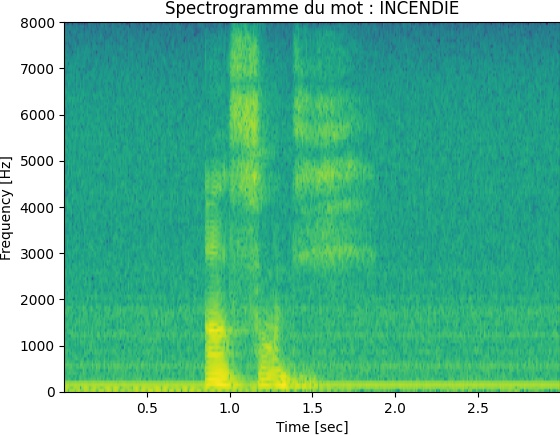
\includegraphics[width=\textwidth]{1-Incendie.jpg}
			\caption{INCENDIE}
		\end{subfigure}
		\begin{subfigure}[]{0.32\textwidth}
			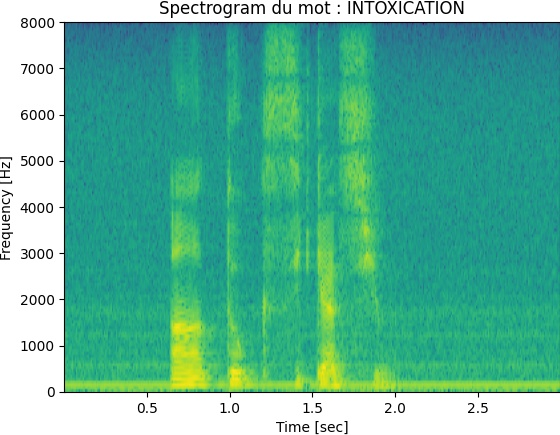
\includegraphics[width=\textwidth]{1-Intoxication.jpg}
			\caption{INTOXICATION}
		\end{subfigure}
		\begin{subfigure}[]{0.32\textwidth}
			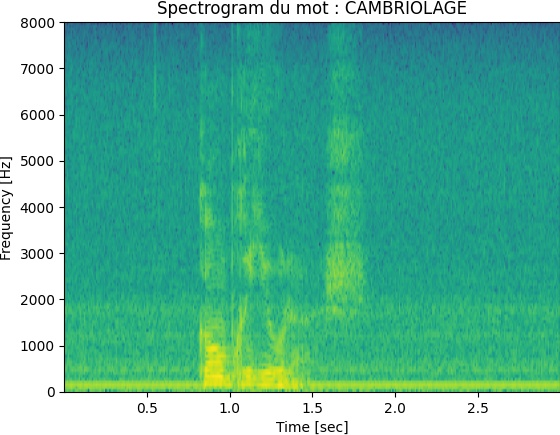
\includegraphics[width=\textwidth]{1-Cambriolage.jpg}
			\caption{CAMBRIOLAGE}
		\end{subfigure}
	\end{figure}
\end{frame}



\begin{frame}{Le découpage en formant}
	\begin{block}{Formant - Définition Larousse}
		Fréquence de résonance du conduit vocal. \\
		Les voyelles se définissent acoustiquement par leurs formants; \\
		seules les consonnes dites vocaliques présentent une structure formantique similaire à celle des voyelles.
	\end{block}
	\begin{figure}
		\begin{center}
			\centering
			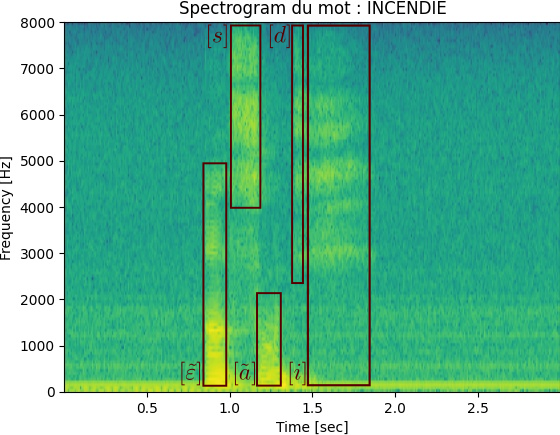
\includegraphics[width=0.45\textwidth]{3-incendie.png}
			\caption{Analyse de formant du mot "INCENDIE" \\avec l'aide de Mme.Voisin en formation d'orthophonie à la Sorbonne}
		\end{center}
	\end{figure}
\end{frame}


% 2-Généralités sur les réseaux de neurones
\section{Généralités sur les réseaux de neurones}
% 2-1 Du perceptron au réseau de neurones
\subsection{Du perceptron au réseau de neurones}

\begin{frame}{Le neurone}
	\begin{block}{Présentation du modèle du perceptron}
		En 1943, McCulloch et Pitts introduisent le modèle du perceptron.  \\
		Ce modèle est basé sur le fonctionnement du neurone humain.
	\end{block}
	\begin{figure}
		\centering
		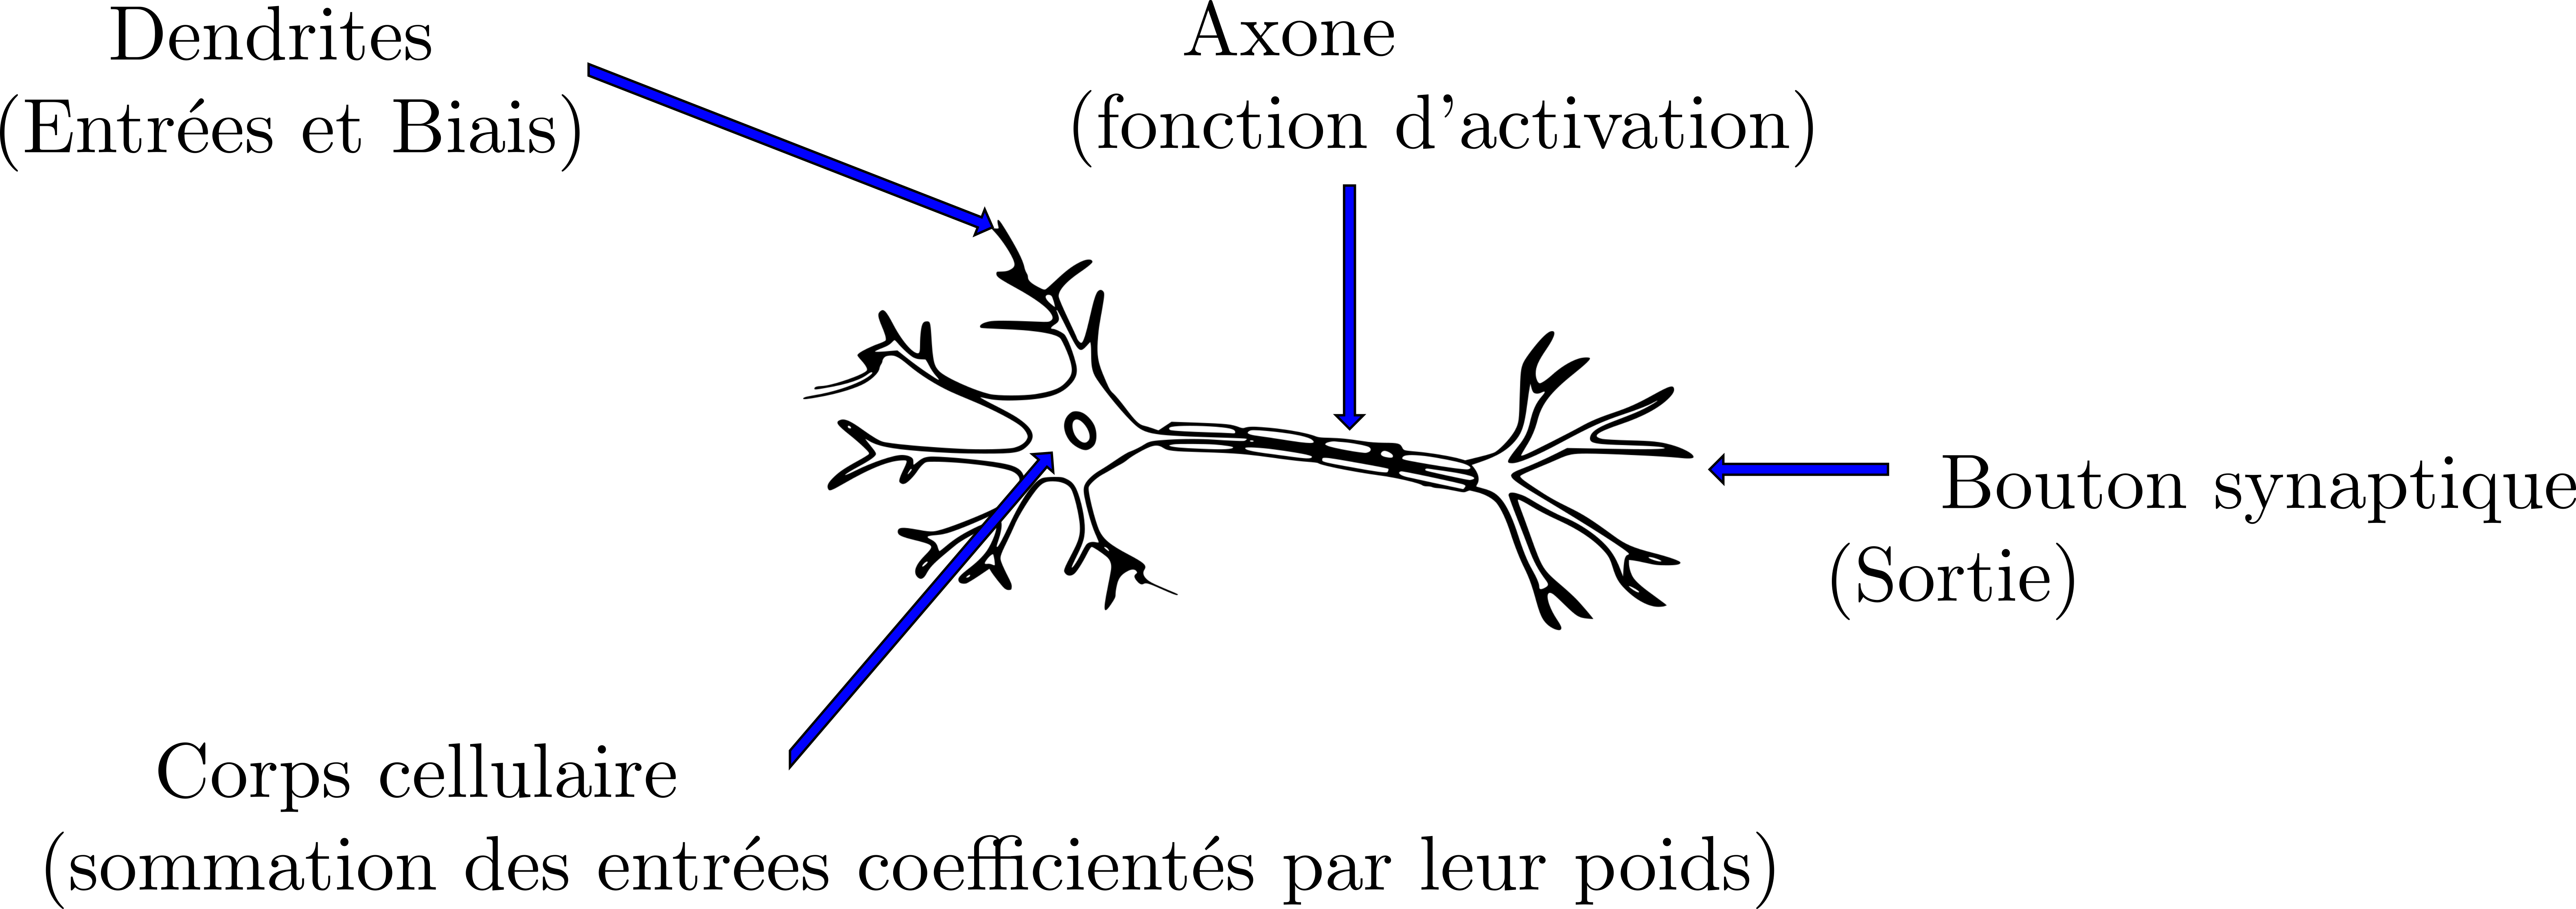
\includegraphics[width=\textwidth]{2-Neurone.png}
		\caption{Schéma d'un neurone humain}
	\end{figure}
\end{frame}

\begin{frame}{Le perceptron}
	\begin{figure}
		\centering
		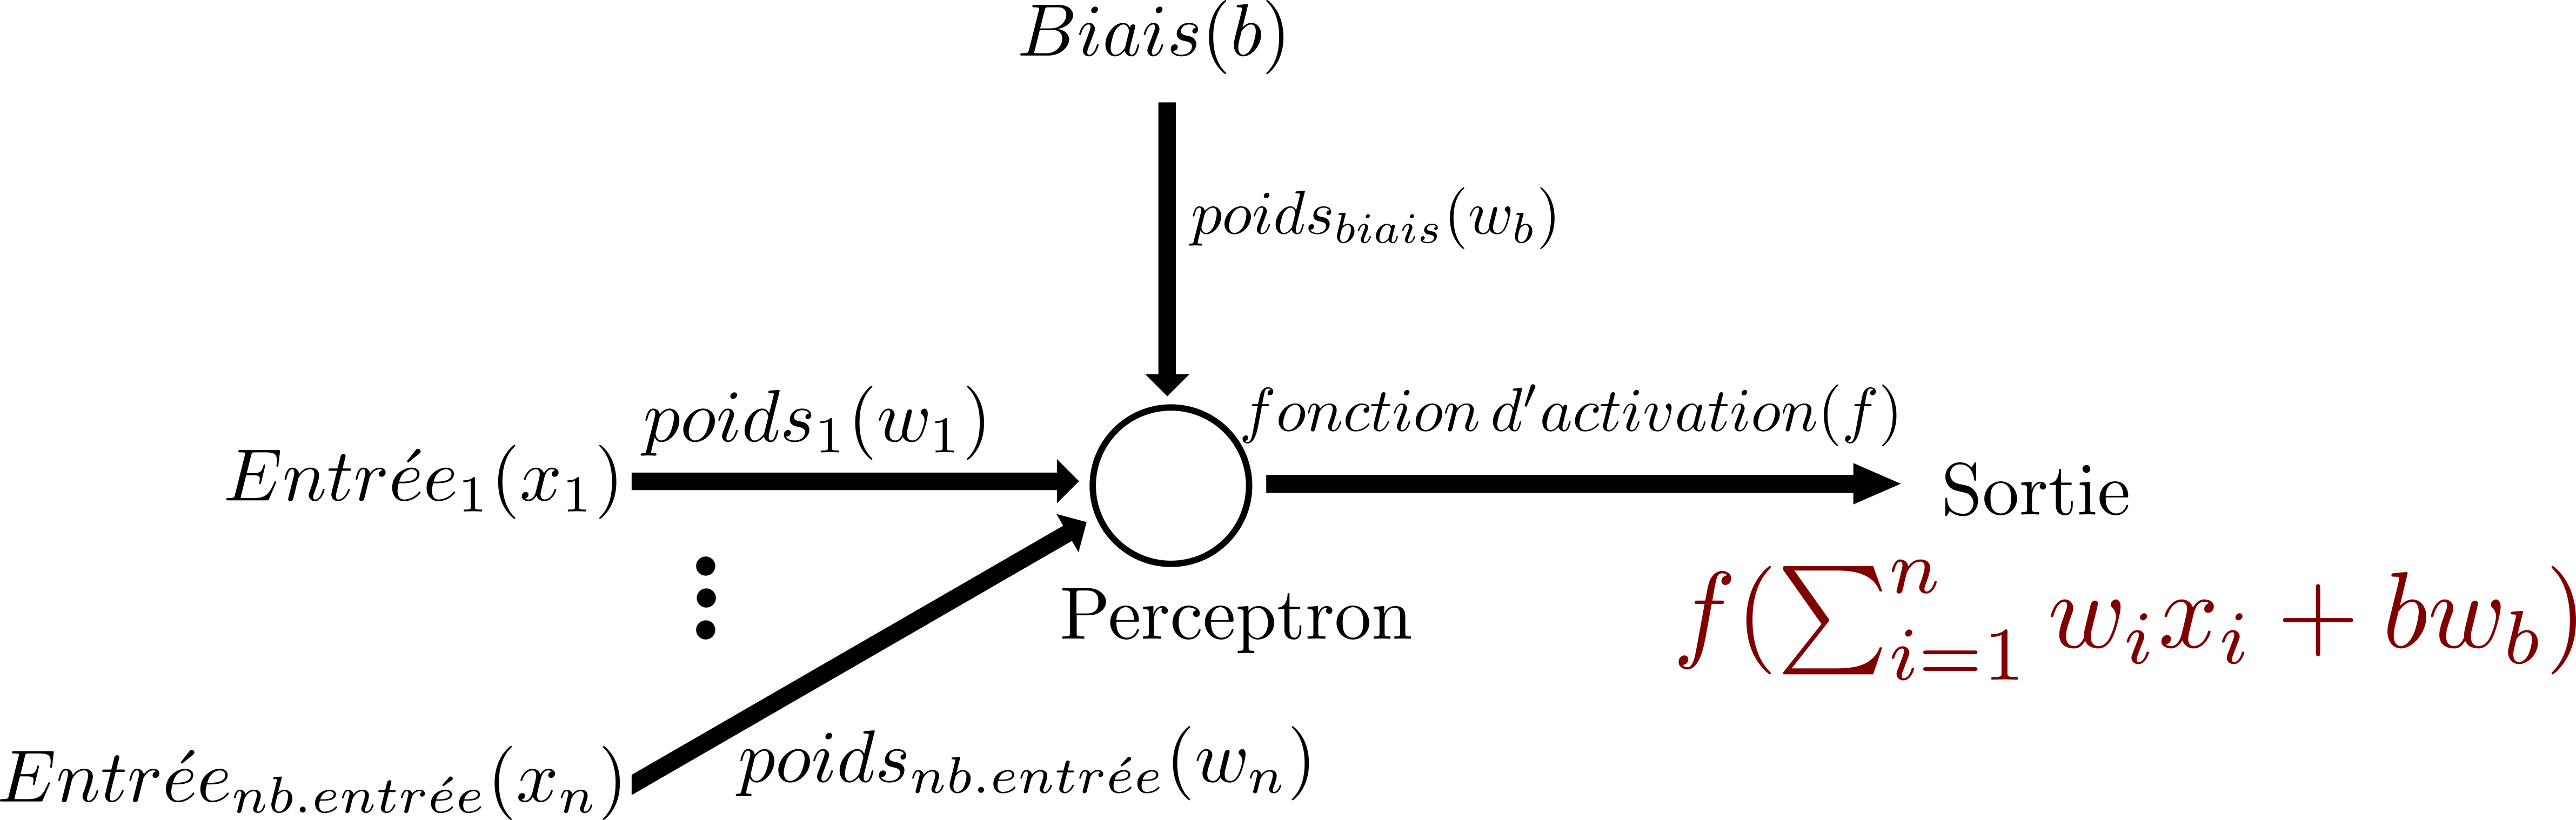
\includegraphics[width=\textwidth]{1-Perceptron.png}
		\caption{Schéma d'un perceptron}
	\end{figure}
\end{frame}


\begin{frame}{Sa représentation informatique}
	\begin{columns}
		\begin{column}[]{0.4\textwidth}
			\begin{center}
				$
					f
					\left(
					\begin{pmatrix}
						x_1 & \ldots & x_n & b
					\end{pmatrix}
					\times
					\begin{pmatrix}
						w_1    \\
						\vdots \\
						w_n    \\
						w_b
					\end{pmatrix}
					\right)
				$ \\
			\end{center}
		\end{column}
		\begin{column}[]{0.5\textwidth}
			\lstinputlisting[language=Python, firstline=15]{0-representation.py}
		\end{column}
	\end{columns}
\end{frame}


\begin{frame}{La fonction d'activation Sigmoïde}
    \begin{center}
        \centering
		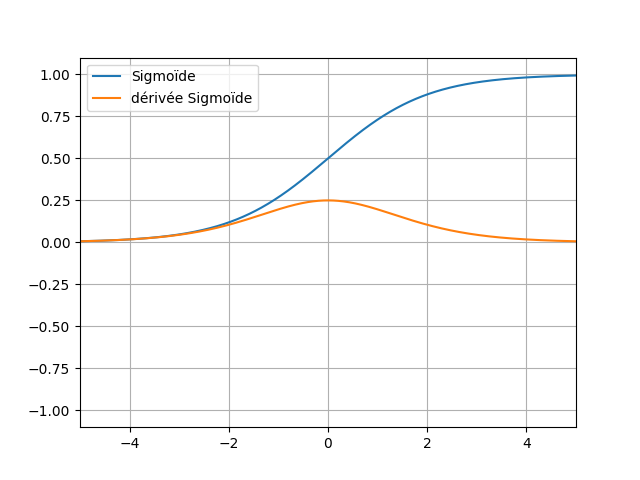
\includegraphics[width=200px]{0-Sigmoide.png} \\~\\
        Sigmoïde : $\mathlarger{\frac{1}{1+e^{-x}}}$ \\~\\
        Dérivée : $f(x) \times (1-f(x))$
    \end{center}   
\end{frame}

\begin{frame}{Le réseau de neurones}
    \begin{figure}
        \centering
        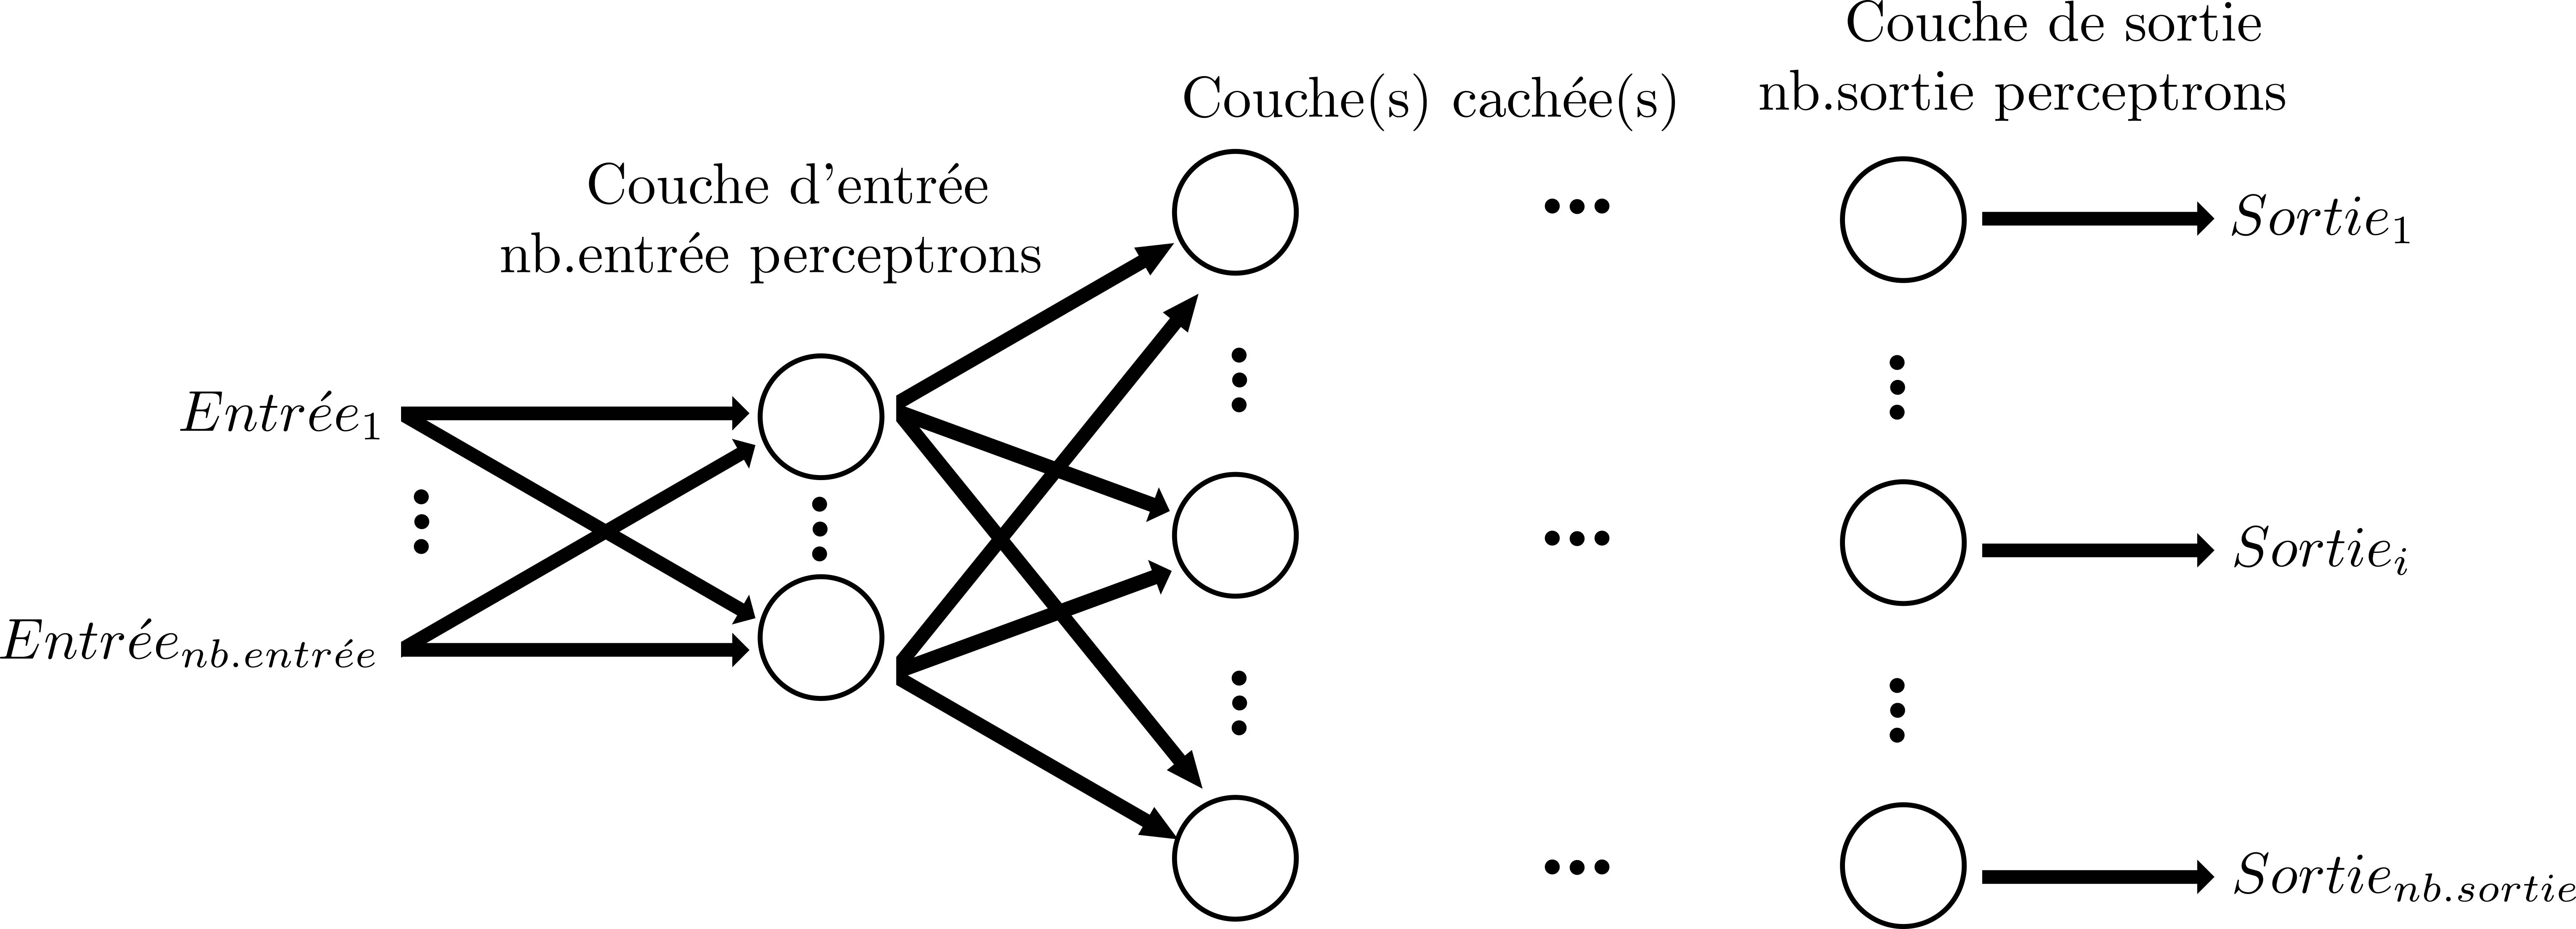
\includegraphics[width=\textwidth]{3-Reseau}
        \caption[]{Schéma d'un réseau de neurones}
    \end{figure}
\end{frame}
% 2-2 Rétropropagation
\subsection{Rétropropagation}

\begin{frame}{La descente de gradient}
    \begin{block}{Descente de gradient}
        Algorithme permettant de converger vers un minimum local d'une fonction. \\
        Elle est utilisée pour trouver le minimum d'une fonction évaluant l'erreur entre la valeur de sortie du réseau de neurones et celle attendue: \\
        \begin{center}
            $f : s \mapsto (s - s_{attendue})^2$\\
        \end{center}
        - $s$ la sortie donnée par le modèle \\
        - $s_{attendue}$ la sortie cible. \\

    \end{block}
    \begin{exampleblock}{Objectif}
        Trouver les paramètres pour annuler la fonction d'erreur revient à résoudre le problème qu'elle évalue.
    \end{exampleblock}
\end{frame}


\begin{frame}{Un exemple d'un perceptron seul}
    \begin{figure}
        \centering
        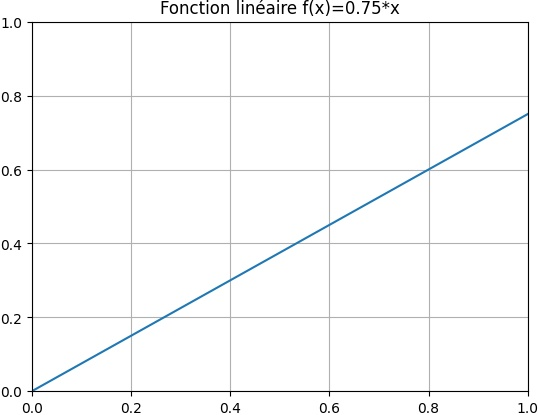
\includegraphics[height=0.5\textheight]{9-fonction_lineaire}
    \end{figure}
    \begin{figure}
        \centering
        
\includegraphics[height=0.2\textheight]{6-Perceptron.png}
        \caption{Schéma d'un perceptron à une entrée}
    \end{figure}
\end{frame}


\begin{frame}{La descente de gradient}
    \begin{block}{Algorithme du gradient}
        $f$ une fonction différentiable de $\mathbb{R} \to \mathbb{R}$. \\
        Soit $x_0$ une valeur initiale aléatoire, $t$ le taux d'apprentissage. \\
        Supposons $x_0, \ldots, x_k$ construits. \\
        • Si $\norme{\nabla f(x_k)} \leq \varepsilon$, on s'arrête. \\
        • Sinon on pose $x_{k+1} = x_k - t \nabla f(x_k)$ \\
    \end{block}
    \begin{figure}
        \centering
        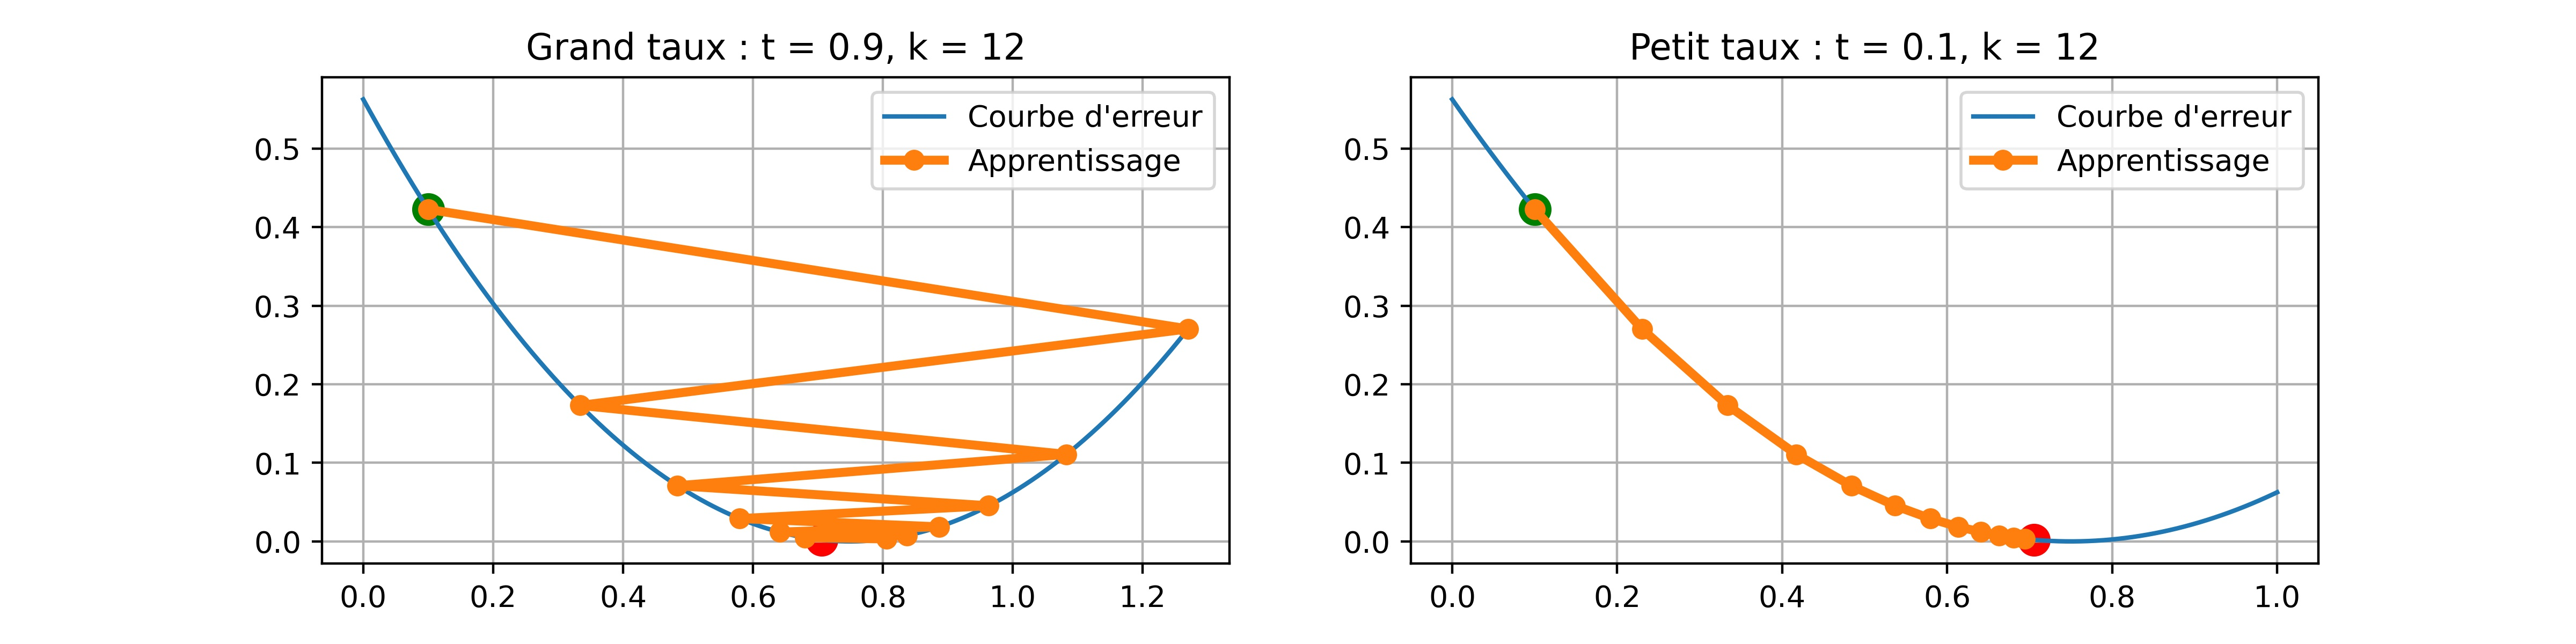
\includegraphics[height=85px]{1-DescenteGradient.jpg}
        \caption{Descente de Gradient pour $f(x) = (x-0.75)^2$; $x_0=0.1$ et $\varepsilon = 0.1$}
    \end{figure}
\end{frame}



% 2-3 Amélioration de la rétropropagation
\subsection{Amélioration de la rétropropagation}



\begin{frame}{La quantité de mouvement (momentum)}
    \begin{block}{Descente de gradient avec momentum}
        $x_0$ aléatoire, momentum $\omega_0 = 0$.
        $x_0, \ldots, x_k$ et $\omega_0, \ldots, \omega_k$ construits. \\
        • On pose $\omega_{k+1} = \gamma \omega_k + t \nabla f(x_k)$ \\
        • On pose $x_{k+1} = x_k - \omega_{k+1}$
    \end{block}
    \begin{figure}
        \centering
        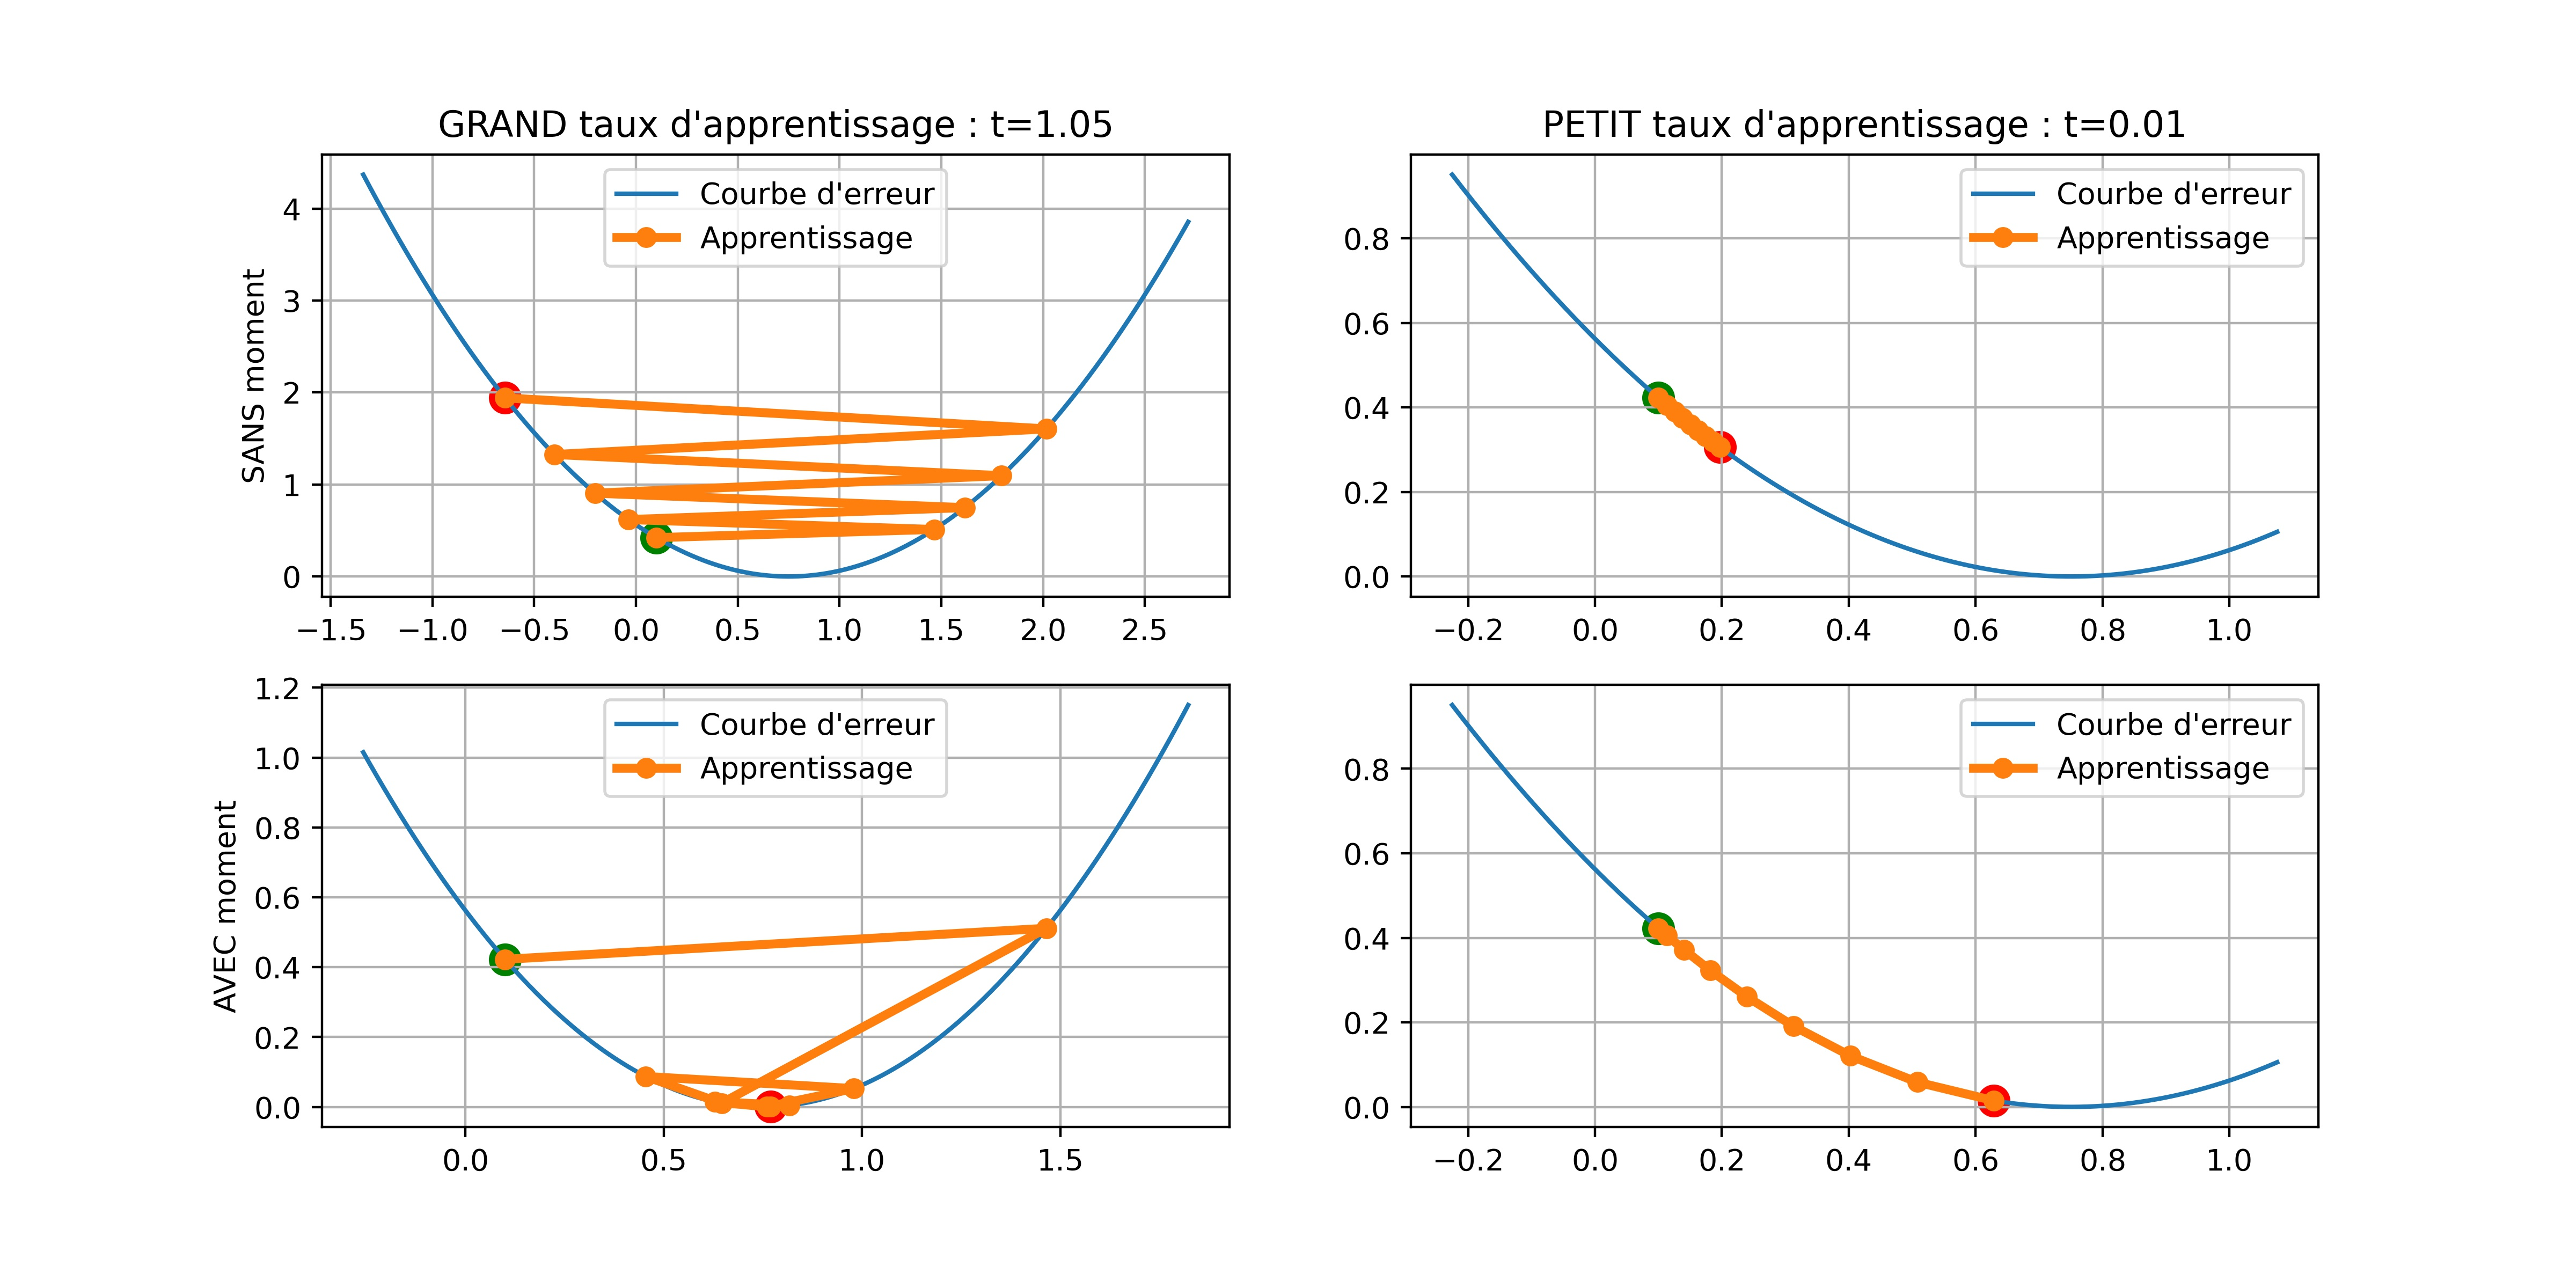
\includegraphics[height=120px]{4-Moment.jpg}
        \caption{Descente de gradient SANS/AVEC momentum où $\gamma = 0.5$}
    \end{figure}
\end{frame}



\begin{frame}{Les avantages du momentum}
    \begin{exampleblock}{Avantages}
        \begin{itemize}
            \item La descente de gradient avec momentum converge plus rapidement
            \item La descente de gradient avec momentum s'échappe de certains minima locaux  
        \end{itemize}  
    \end{exampleblock}
    \begin{figure}
        \centering
        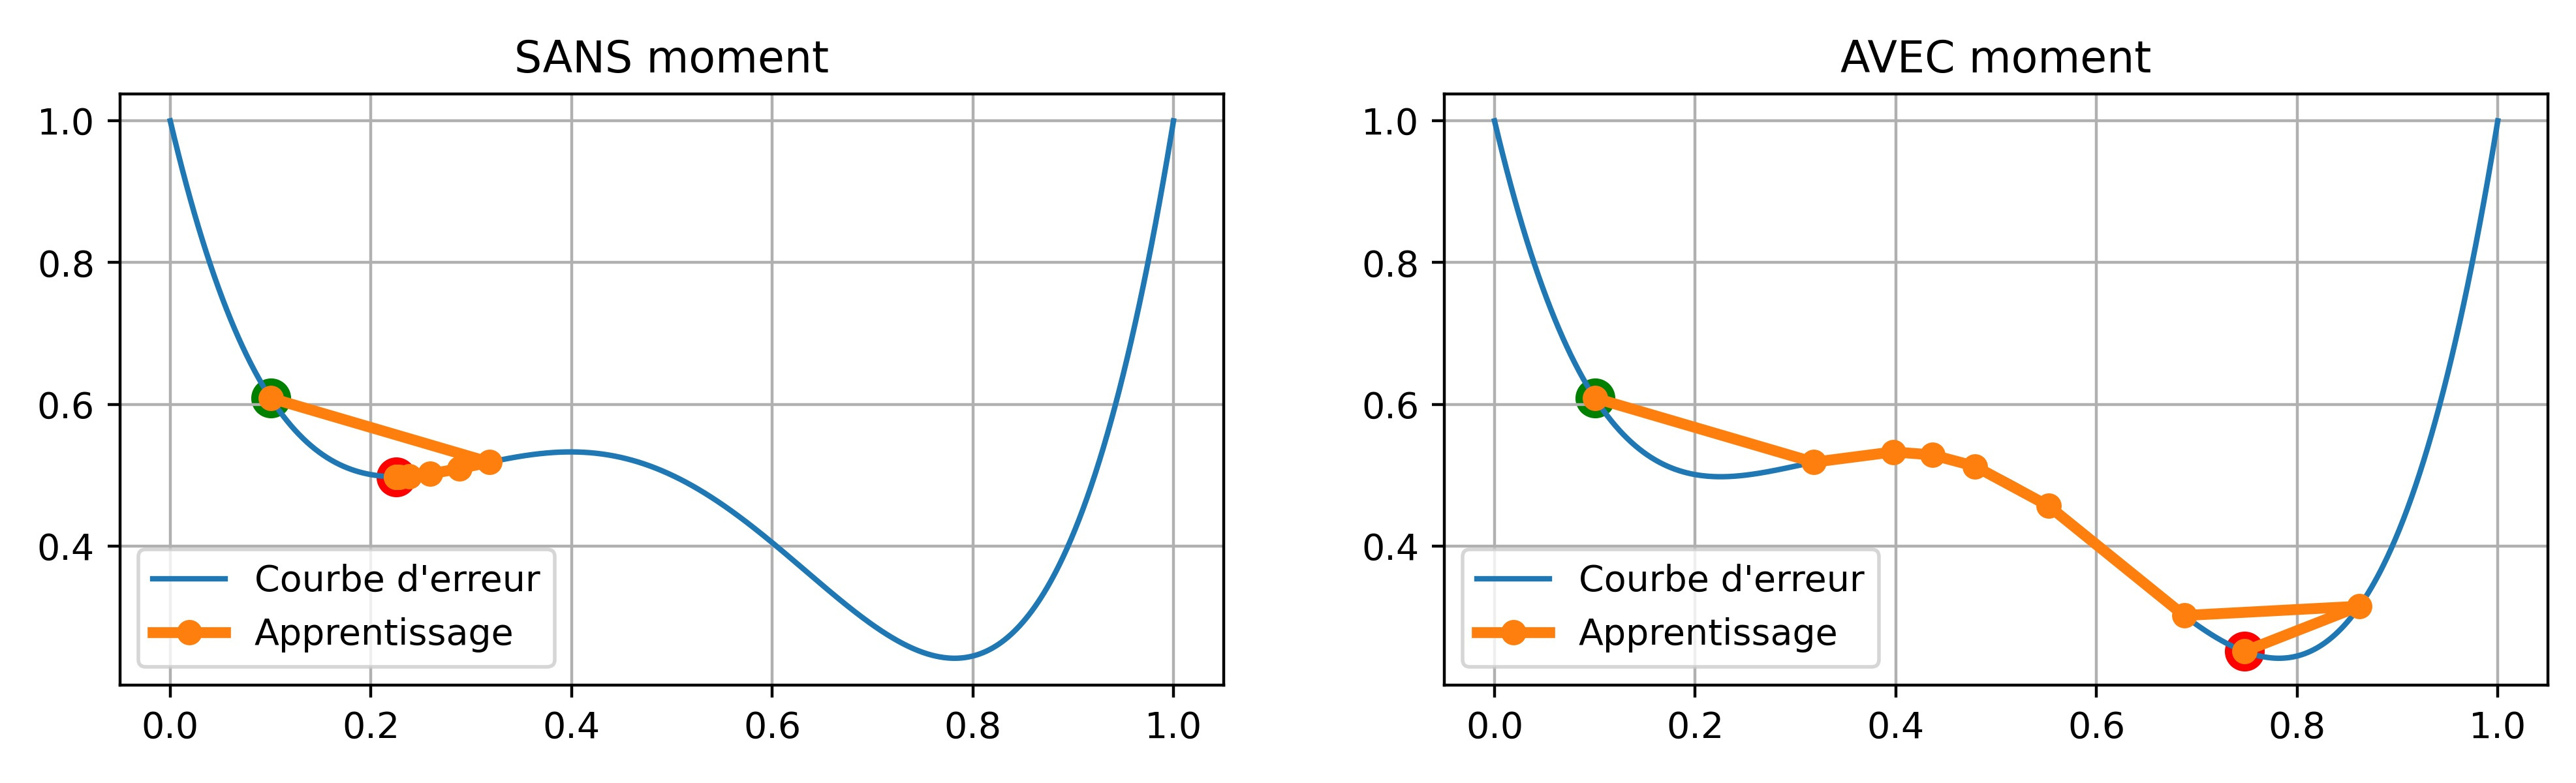
\includegraphics[width=\textwidth]{5-Moment.jpg}
        \caption{Descente de gradient SANS/AVEC momentum où $\gamma = 0.5$}
    \end{figure}
\end{frame}




\begin{frame}{L'apprentissage stochastique ou par paquet (batch)}
    \begin{alertblock}{Problème d'incertitude des données}
        Les données d'apprentissage ne sont pas toujours exactes. \\
        J'ajoute donc aux données théoriques une valeur d'incertitude, pour se rapprocher au plus de la réalité. 
    \end{alertblock}
    \begin{exampleblock}{Solution}
        Il est alors préférable d'appliquer la rétropropagation à notre réseau sur des paquets de données plutôt que donnée par donnée. 
    \end{exampleblock}
    \begin{center}
        \centering
        $
            \left< f
            \left(
            \begin{pmatrix}
                    x_1^{1} & \ldots & x_n^{1} & b      \\
                    \vdots  & \vdots & \vdots  & \vdots \\
                    x_1^{D} & \ldots & x_n^{D} & b
                \end{pmatrix}
            \times
            \begin{pmatrix}
                    w_1    \\
                    \vdots \\
                    w_n    \\
                    w_b
                \end{pmatrix}
            \right) \right>
        $
    \end{center}
\end{frame}


\begin{frame}{Une illustration de l'apprentissage par batch}
    \begin{figure}
        \centering
        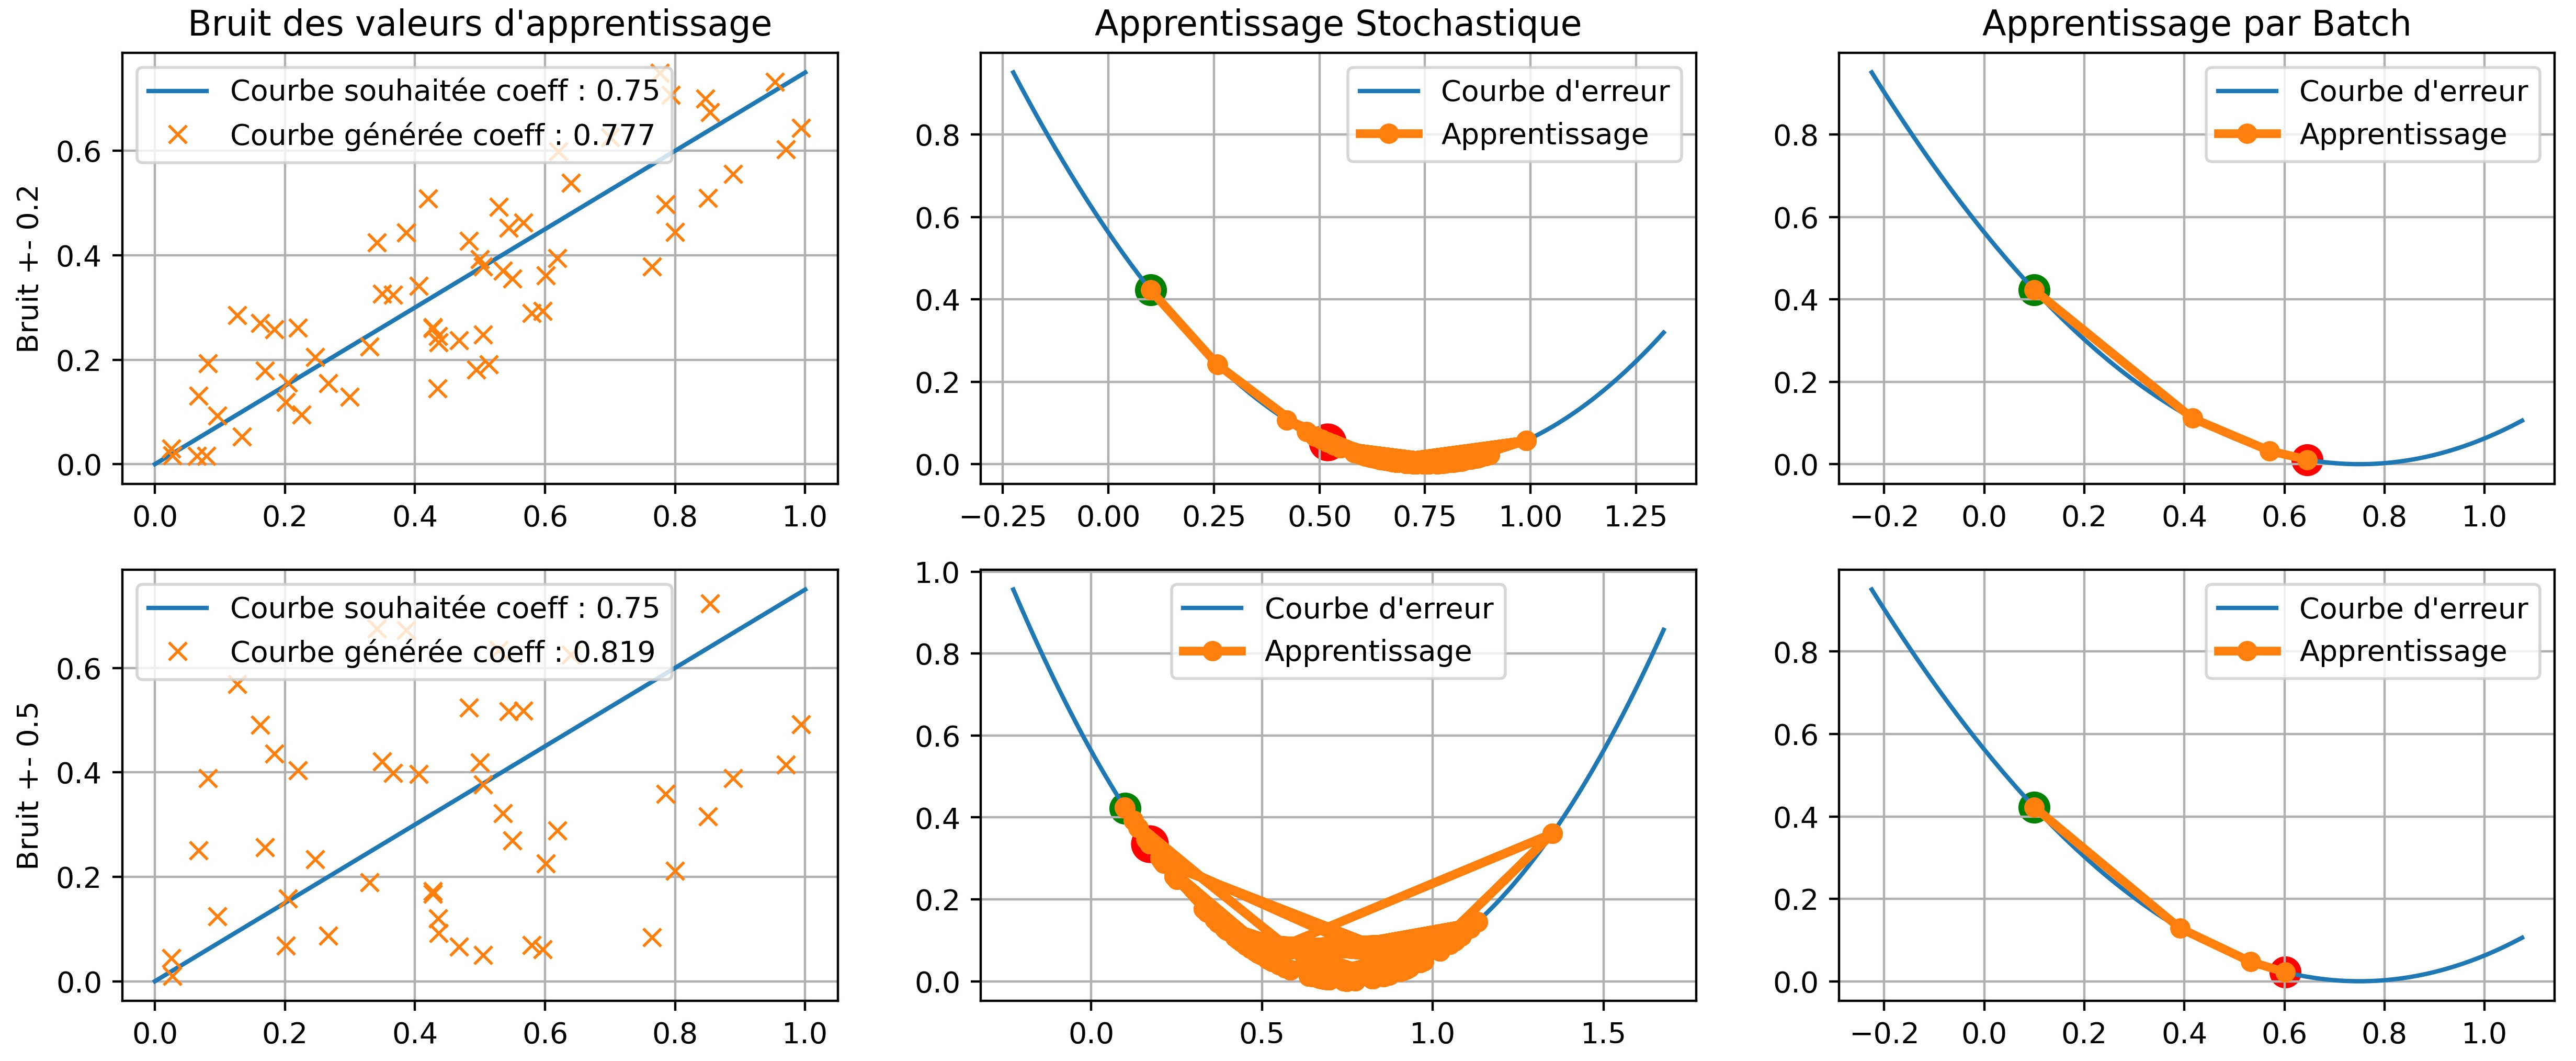
\includegraphics[width=\textwidth]{7-Batch.jpg}
        \caption{Comparaison apprentissage stochastique et par paquet}
    \end{figure}
\end{frame}


% 3 Réalisations concrètes
\section{Réalisations concrètes}
% 3-1 Reproduction du XOR
\subsection{Reproduction du XOR}

\begin{frame}{L'opérateur XOR}
	\begin{block}{Le XOR nécessite un réseau}
		Le XOR, \og $ou\ exclusif$ \fg, est un opérateur non linéairement séparable. \\
	\end{block}
    \begin{columns}
        \begin{column}{0.6\textwidth}
            \begin{figure}
                \centering
                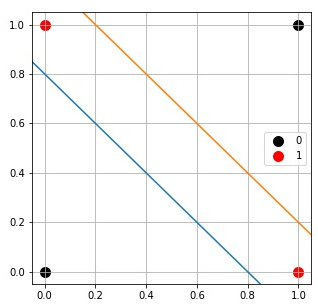
\includegraphics[width=150px]{2-XOR.jpg}
                \caption{Schéma de l'opérateur XOR}
            \end{figure}
        \end{column}
        \begin{column}[]{0.3\textwidth}
            \begin{center}
                \begin{tabular}{|c c | c|}
                    \hline
                    A & B & A xor B \\ \hline
                    0 & 0 & 0 \\
                    0 & 1 & 1 \\
                    1 & 0 & 1 \\
                    1 & 1 & 0 \\
                    \hline
                \end{tabular}
                \end{center}
        \end{column}
    \end{columns}
\end{frame}



\begin{frame}{Le réseau de neurone reproduisant l'opérateur XOR}
	\begin{figure}
		\centering
		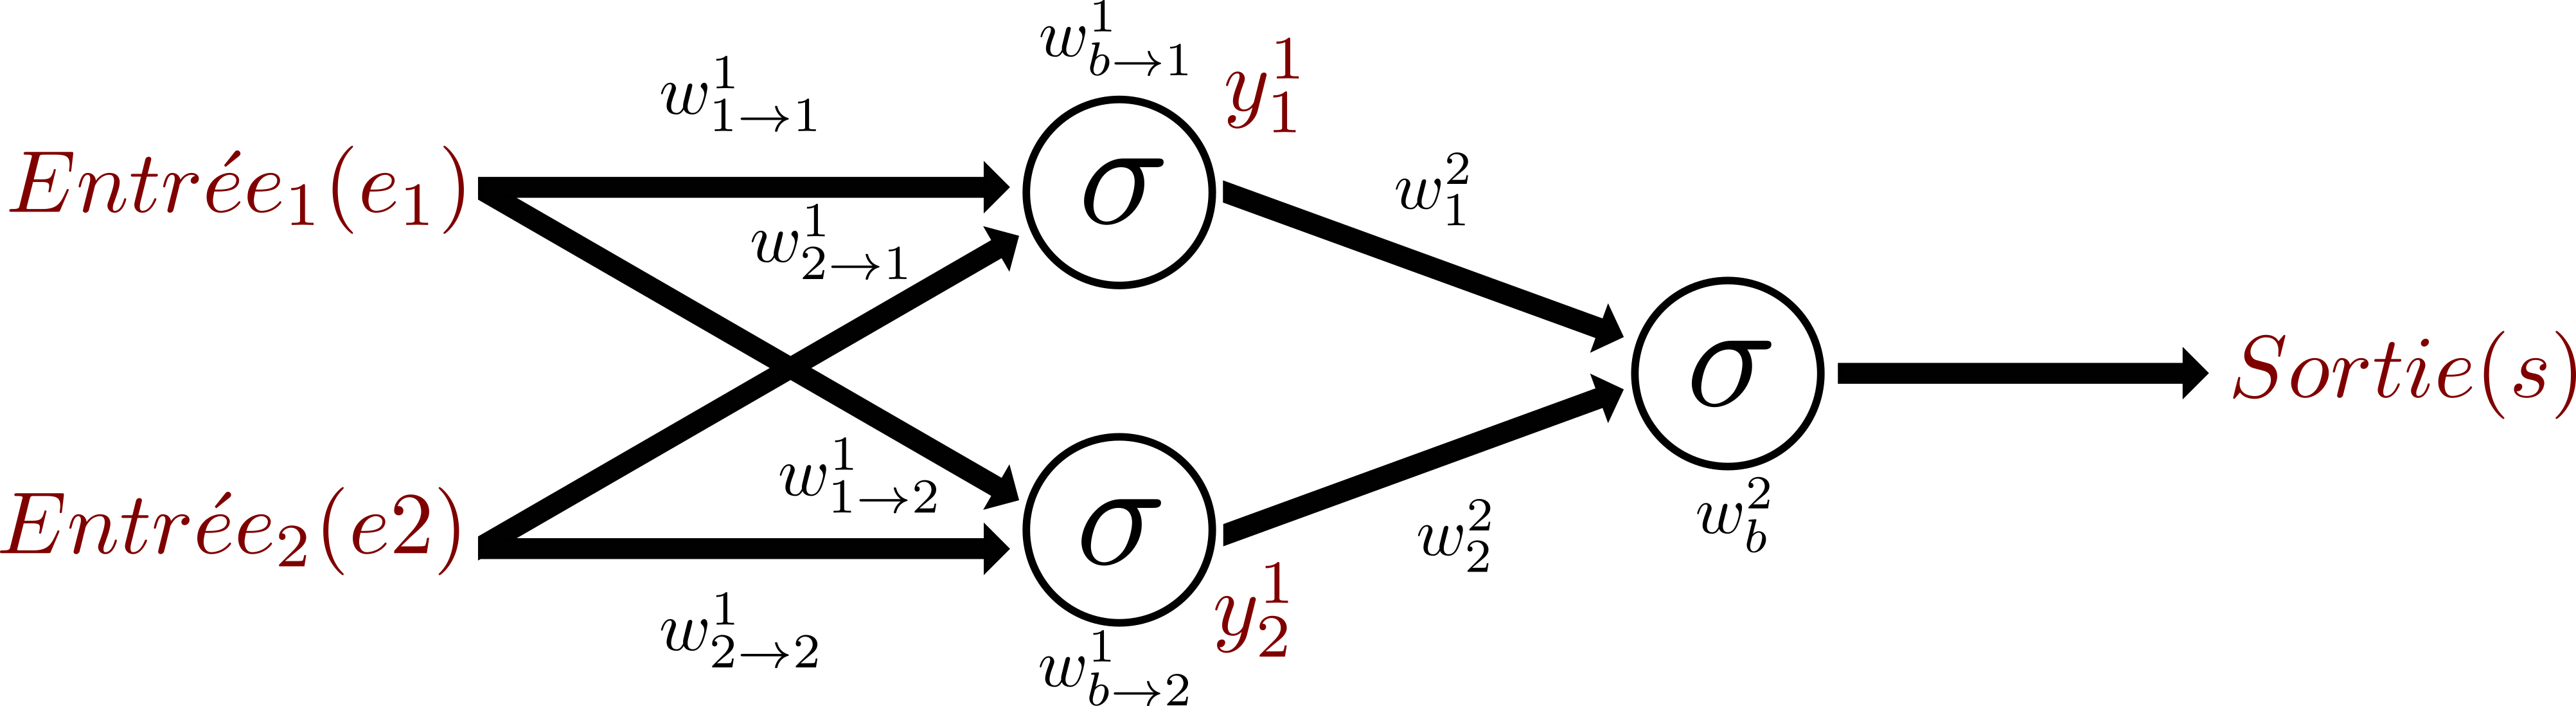
\includegraphics[width=\textwidth]{3-Model.png}
		\caption{Schéma du réseau de neurone reproduisant le XOR}
	\end{figure}
\end{frame}

\begin{frame}{L'apprentissage de la reproduction du XOR}
	\begin{figure}
		\centering
		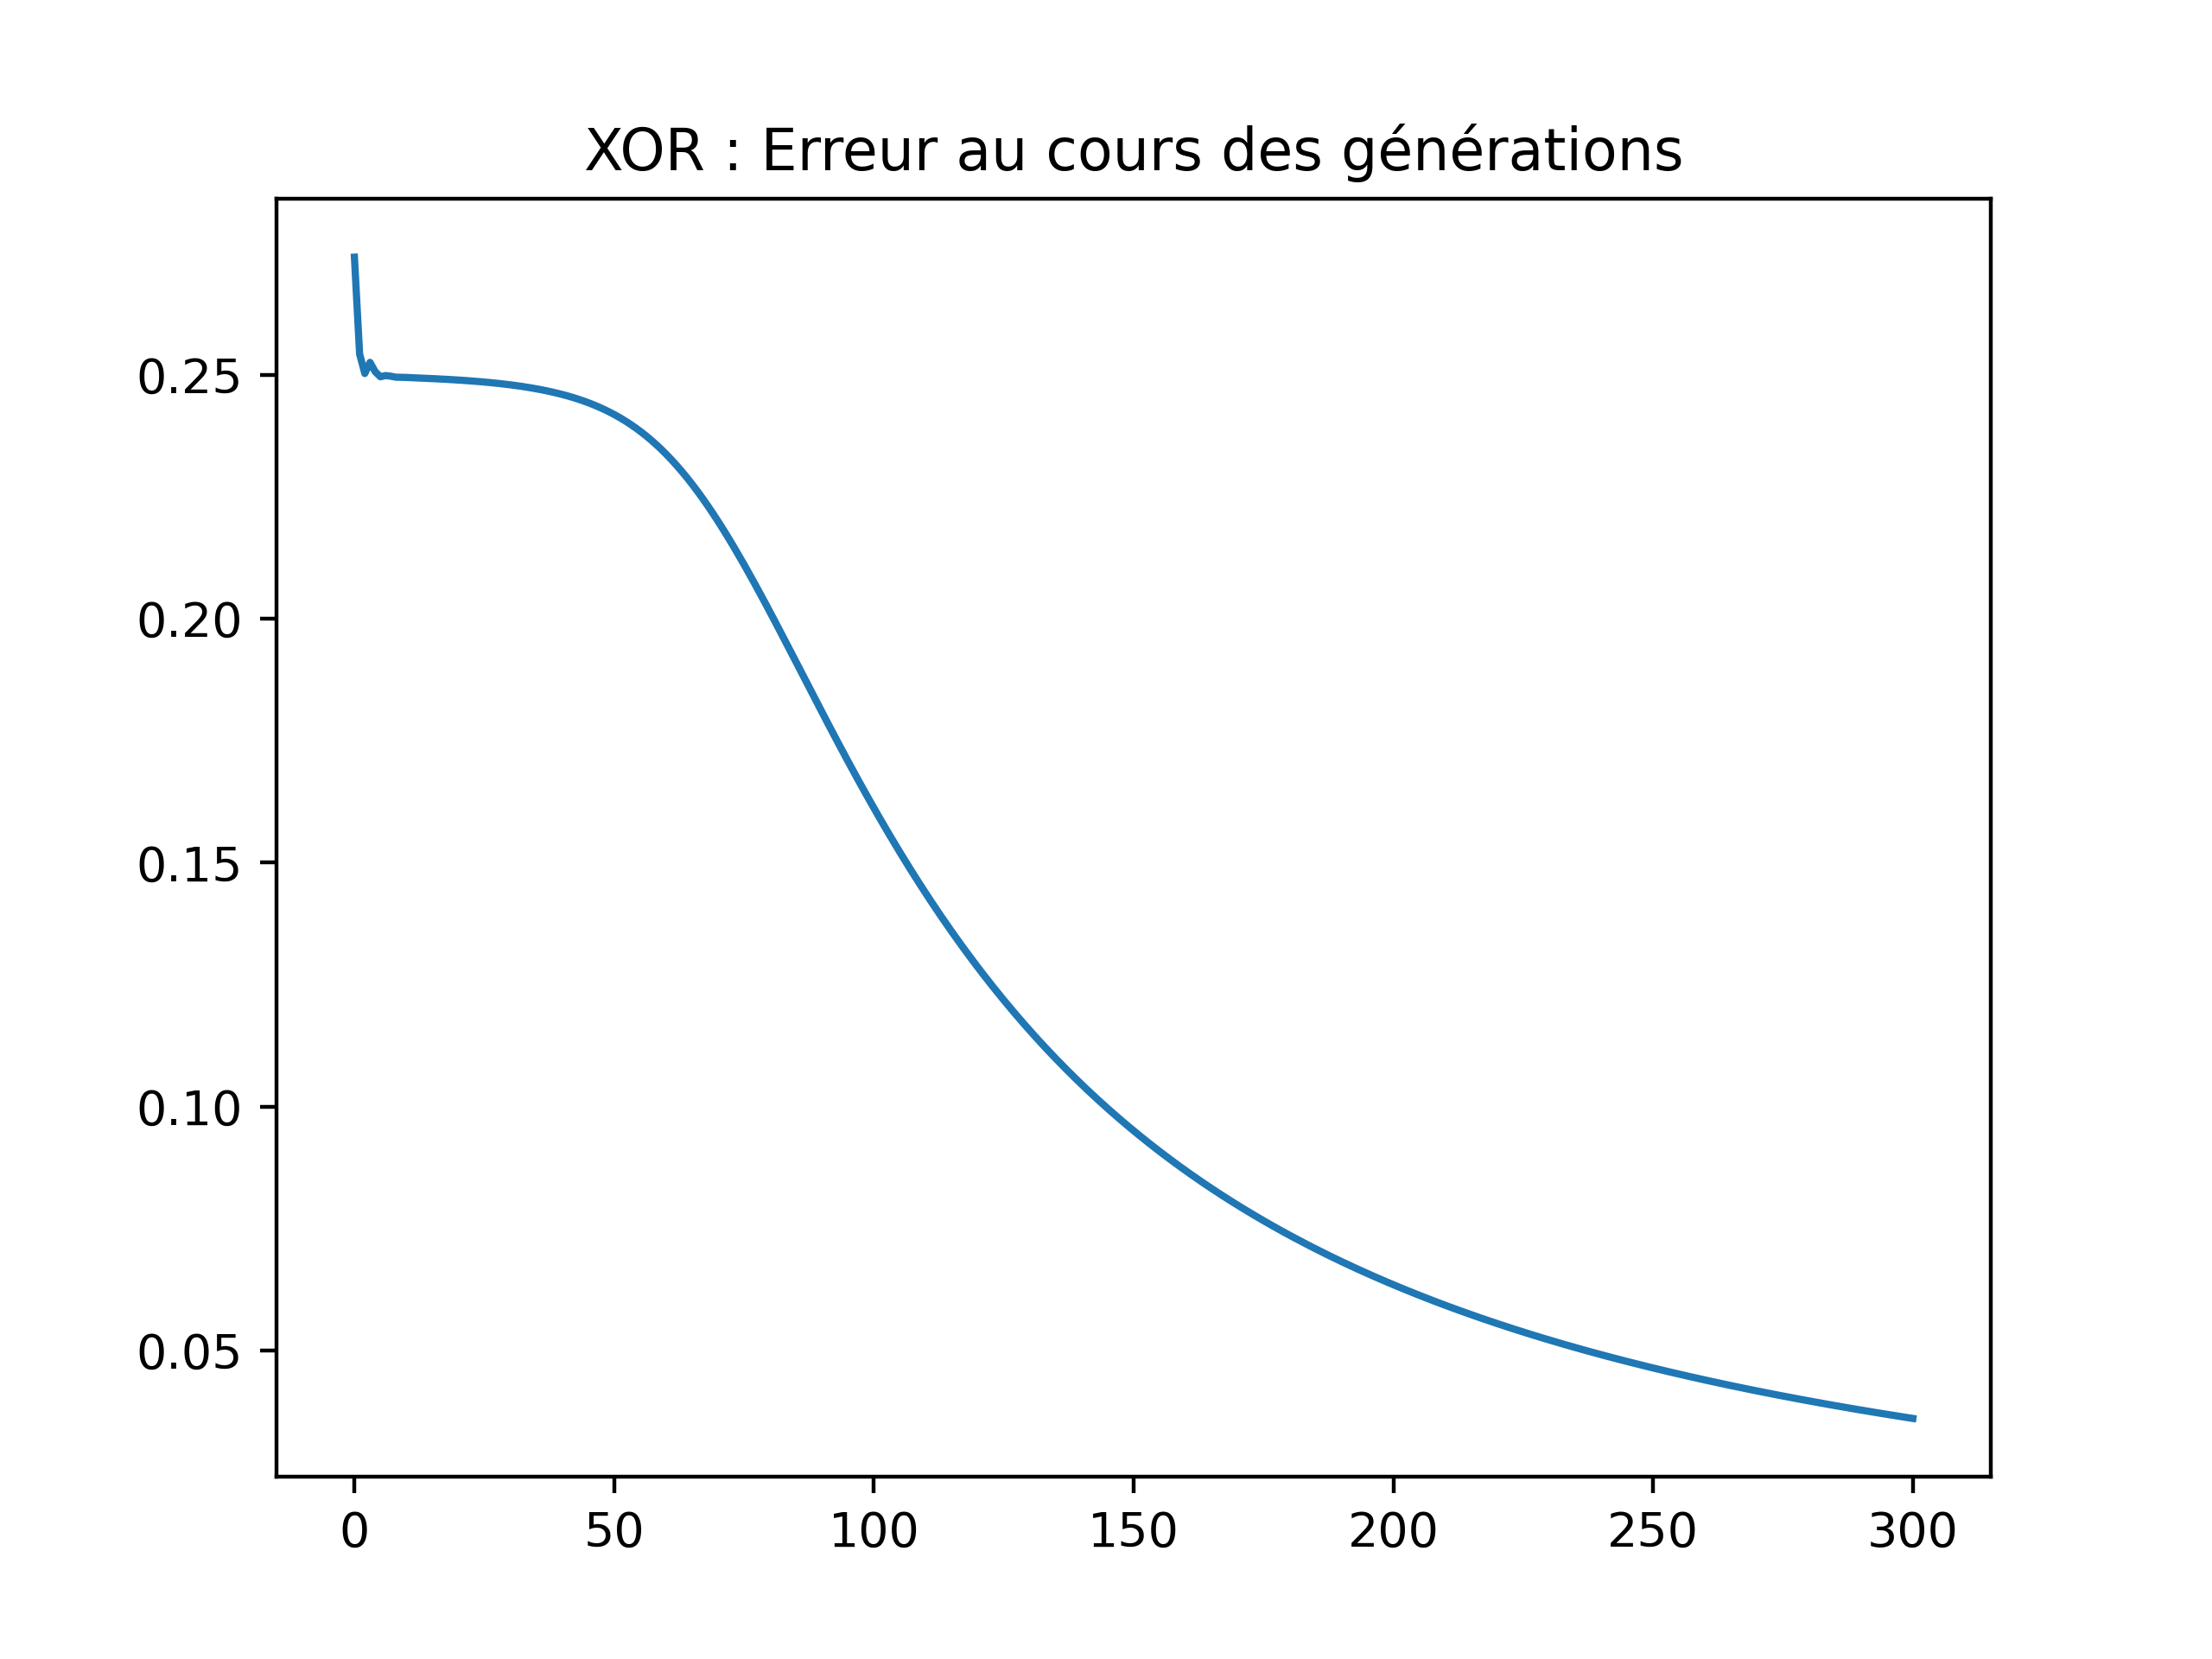
\includegraphics[width=270px]{4-XOR.png}
		\caption{Erreur sur la reproduction du XOR au cours de l'apprentissage}
	\end{figure}
\end{frame}


\begin{frame}{IV - Mes résultat}
	\begin{block}{Données}
		• 4 données \\
		• 300 générations
	\end{block}
	\begin{align*}
		Entr\acute{e} e\, :
		\begin{pmatrix}
			0 & 0 \\
			0 & 1 \\
			1 & 0 \\
			1 & 1
		\end{pmatrix}
		 & \to
		\mathlarger{\mathlarger{\sigma_{couche1}}}
		\left( \centerdot \times
		\begin{pmatrix}
				0.85 & 5.42 \\
				0.85 & 5.40 
			\end{pmatrix}
		\right) \\
		 & \to
		\mathlarger{\mathlarger{\sigma_{couche2}}}
		\left( \centerdot \times
		\begin{pmatrix}
				-18.39 \\
				14.42  
			\end{pmatrix}
		\right) \\
		 & \to
		Sortie\, :
		\begin{pmatrix}
			0.12 \\
			0.81 \\
			0.81 \\
			0.24
		\end{pmatrix}
		Sortie_{attendue}\, :
		\begin{pmatrix}
			0 \\
			1 \\
			1 \\
			0
		\end{pmatrix}
	\end{align*}
\end{frame}
% 3-2 Reconnaissance de chiffres écrits
\subsection{Reconnaissance de chiffres écrits}

\begin{frame}{La base de données}
	\begin{block}{Description}
		Images de taille $28 \times 28$ pixels en noir et blanc : \\
		\quad - 60 000 images pour l'entrainement. \\
		\quad - 10 000 autres pour la vérification.
	\end{block}
	\begin{figure}
		\centering
		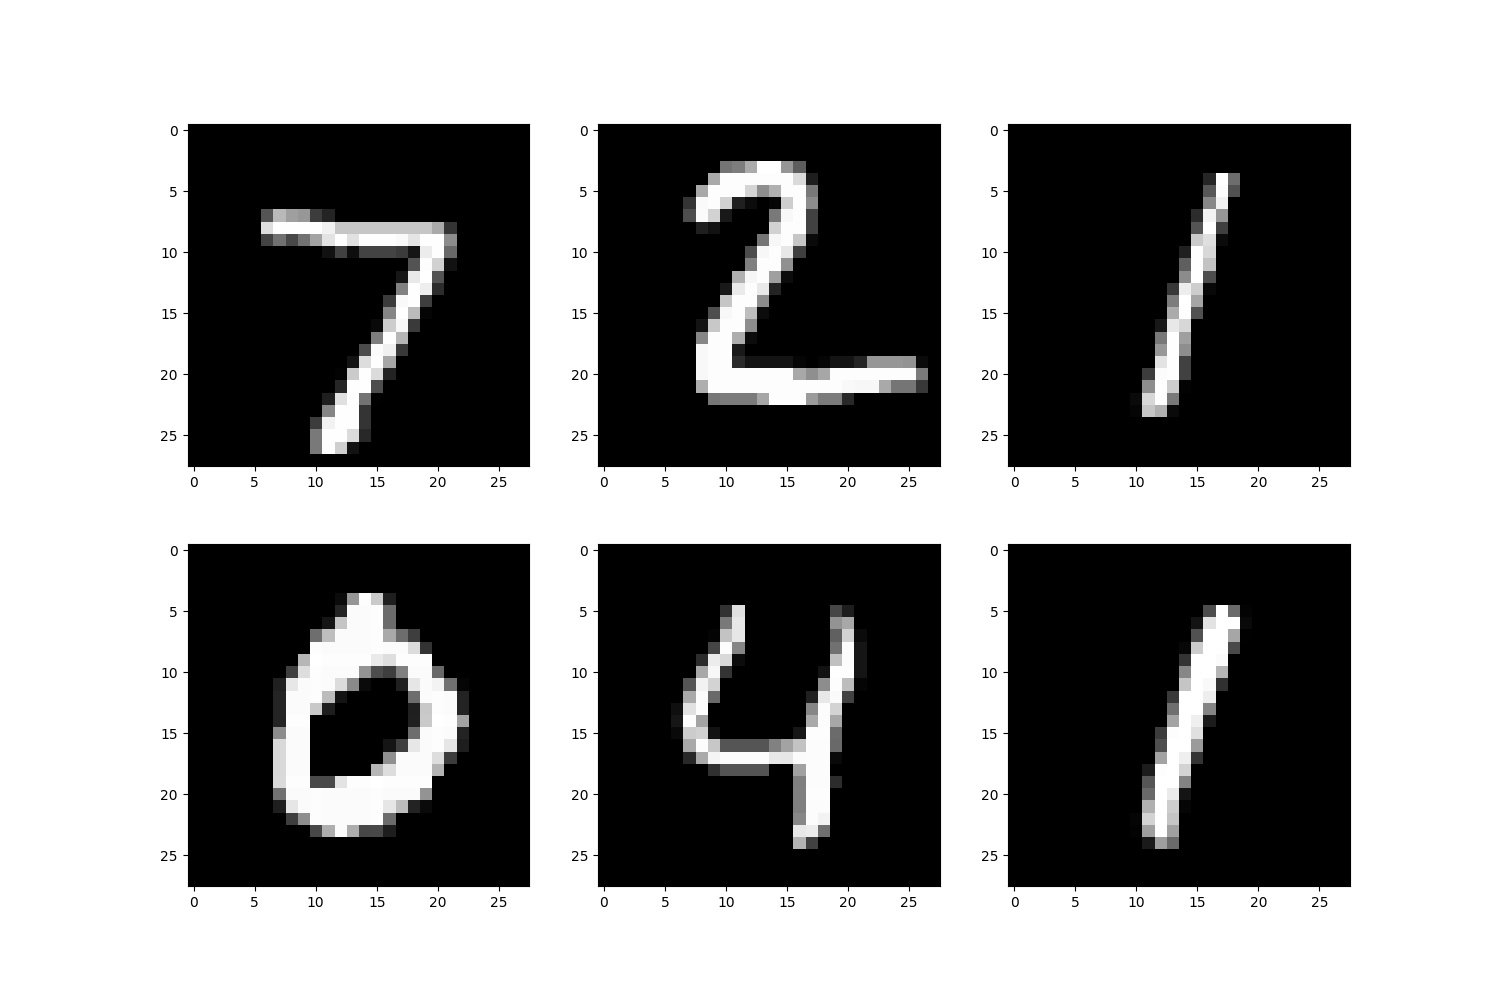
\includegraphics[width=150px]{1-mnist.jpg}
		\caption{Exemple d'images}
	\end{figure}
\end{frame}


\begin{frame}{Un réseau de neurones pour la classification}
	\begin{block}{Softmax}
		La fonction d'activation softmax permet d'obtenir en sortie une distribution de probabilité : \\
		• $p_i = \frac{exp(a_i)}{\sum_{k=1}^{n}exp(a_k)}$ la probabilité de la sortie $a_i$ \\
		• $\dfrac{\partial p_i}{\partial a_j} = p_i\times(\delta_{ij}-p_j)$ \\
	\end{block}
\end{frame}



\begin{frame}{L'utilisation de la fonction Softmax}
	\begin{figure}
		\centering
		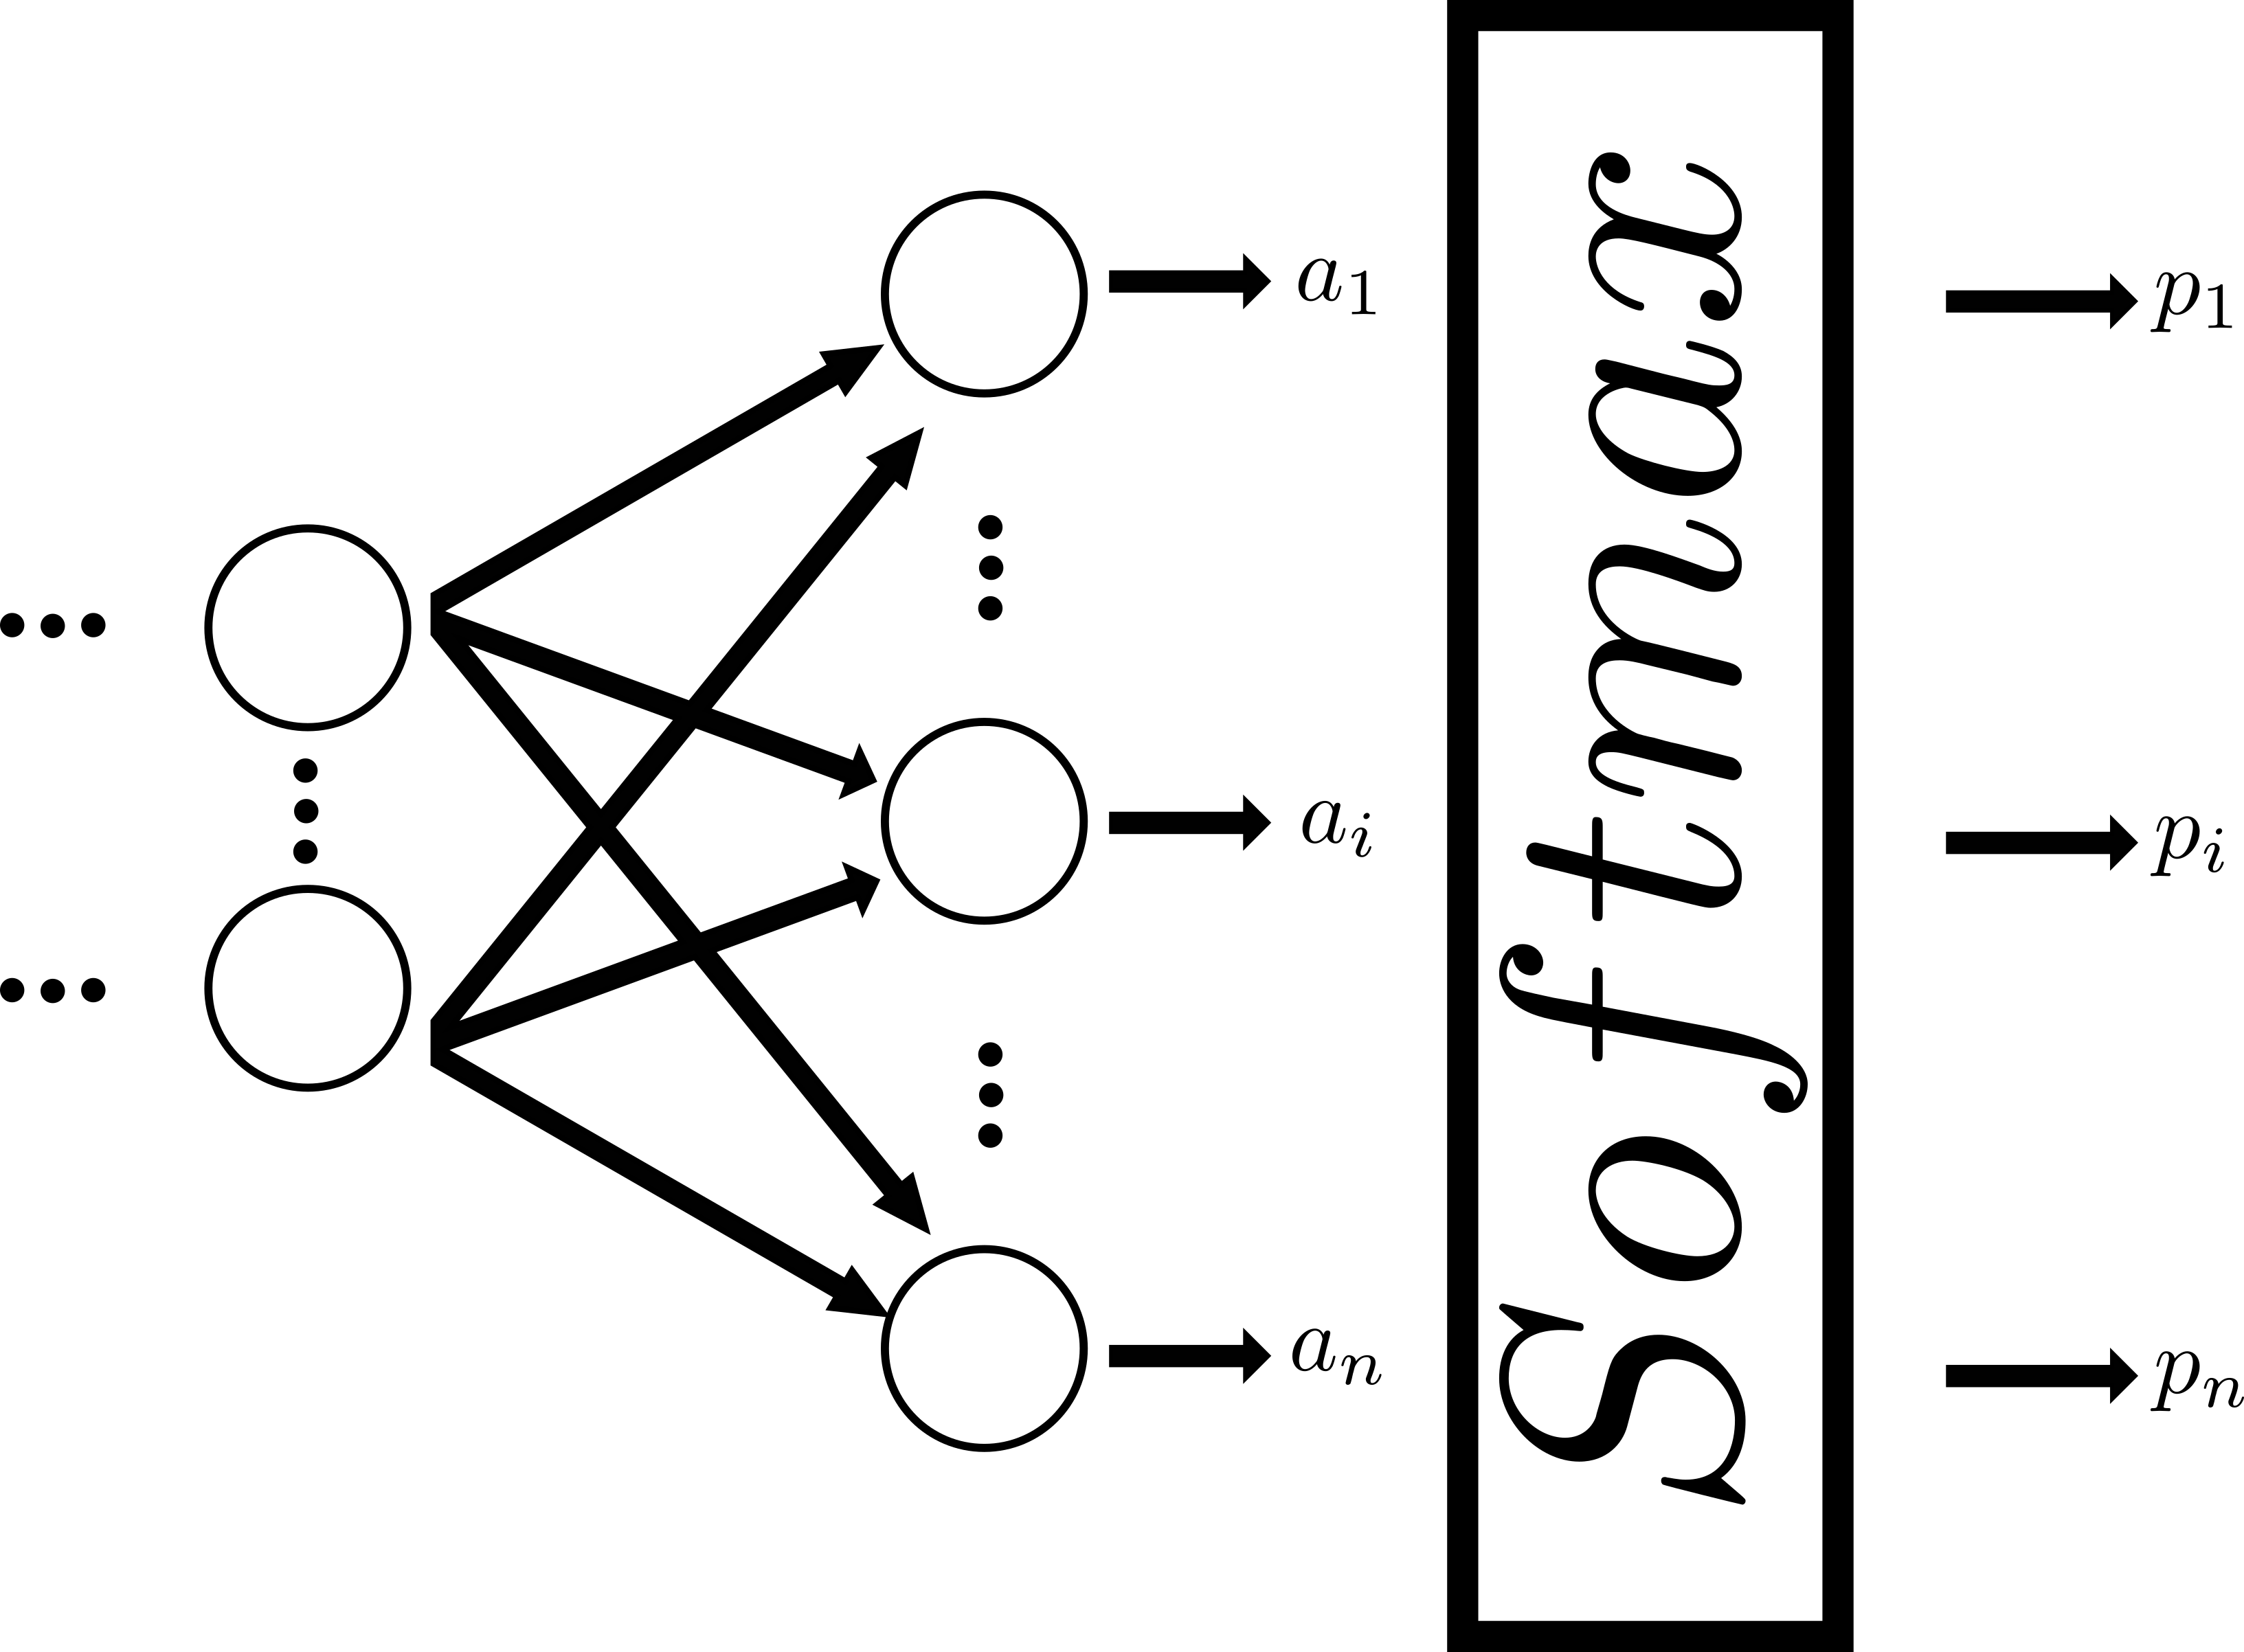
\includegraphics[height=150px]{2-Softmax.png}
		\caption{Schéma d'utilisation du Softmax}
	\end{figure}
\end{frame}


\begin{frame}{La rétropropagation pour la classification}
	\begin{block}{Cross-entropy}
		La fonction d'erreur des problèmes de classification est Cross-entropy : \\
		• $L\ \ \ = -\sum_{k=1}^{n}y_ilog(p_i)$ avec $y_i$ la sortie attendue \\
		• $\dfrac{\partial L}{\partial a_i} = p_i - y_i$
	\end{block}

\end{frame}

\begin{frame}{L'évolution de l'apprentissage}
	\begin{columns}[T] % align columns
		\begin{column}{.58\textwidth}
			\begin{figure}
				\centering
				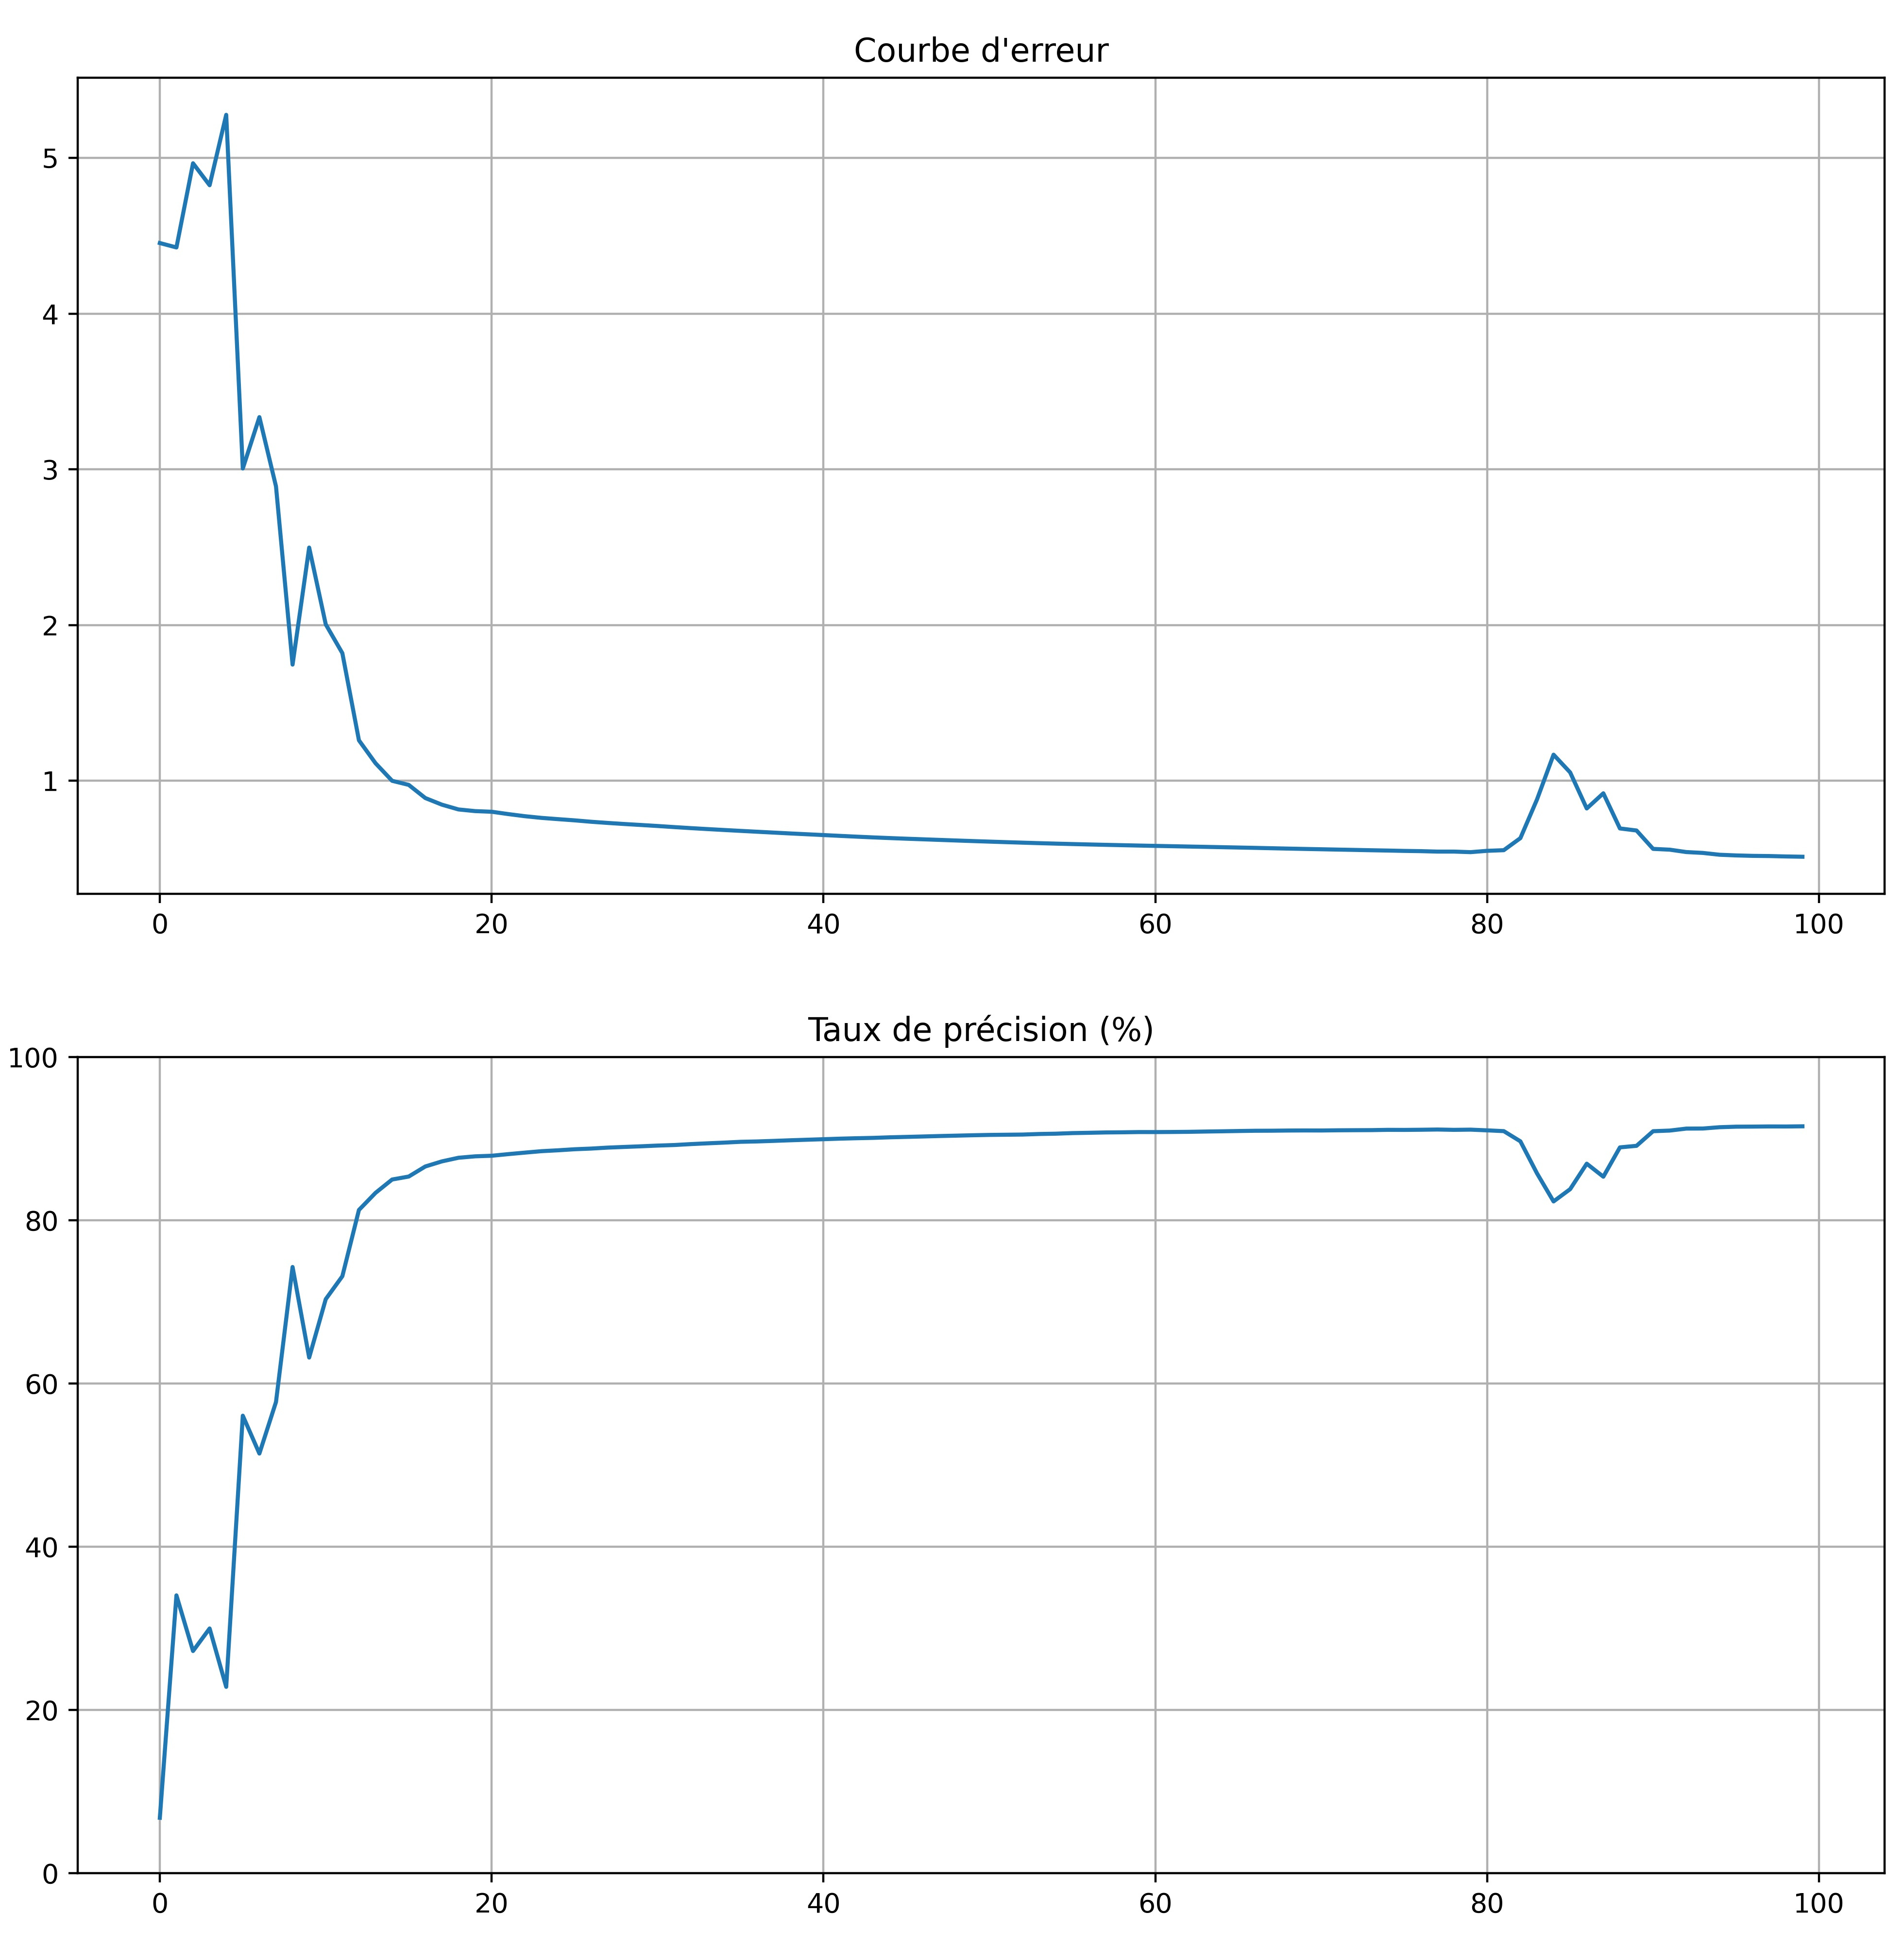
\includegraphics[height=0.7\textheight]{3-Apprentissage.jpg}
				\caption{Courbes d'apprentissage}
			\end{figure}
		\end{column}
		\hfill
		\begin{column}{.54\textwidth}
			\bigskip	\bigskip	\bigskip
			\bigskip	\bigskip	\bigskip
			\bigskip	\bigskip	\bigskip
			Taux de bonnes réponses après 100 générations d'entrainement : \\
			- 91.5\% sur les données d'entrainement \\
			- 91.3\% sur les données de validation. \\
		\end{column}%
	\end{columns}
\end{frame}


\begin{frame}{Mes résultats}
	\begin{figure}
		\centering
		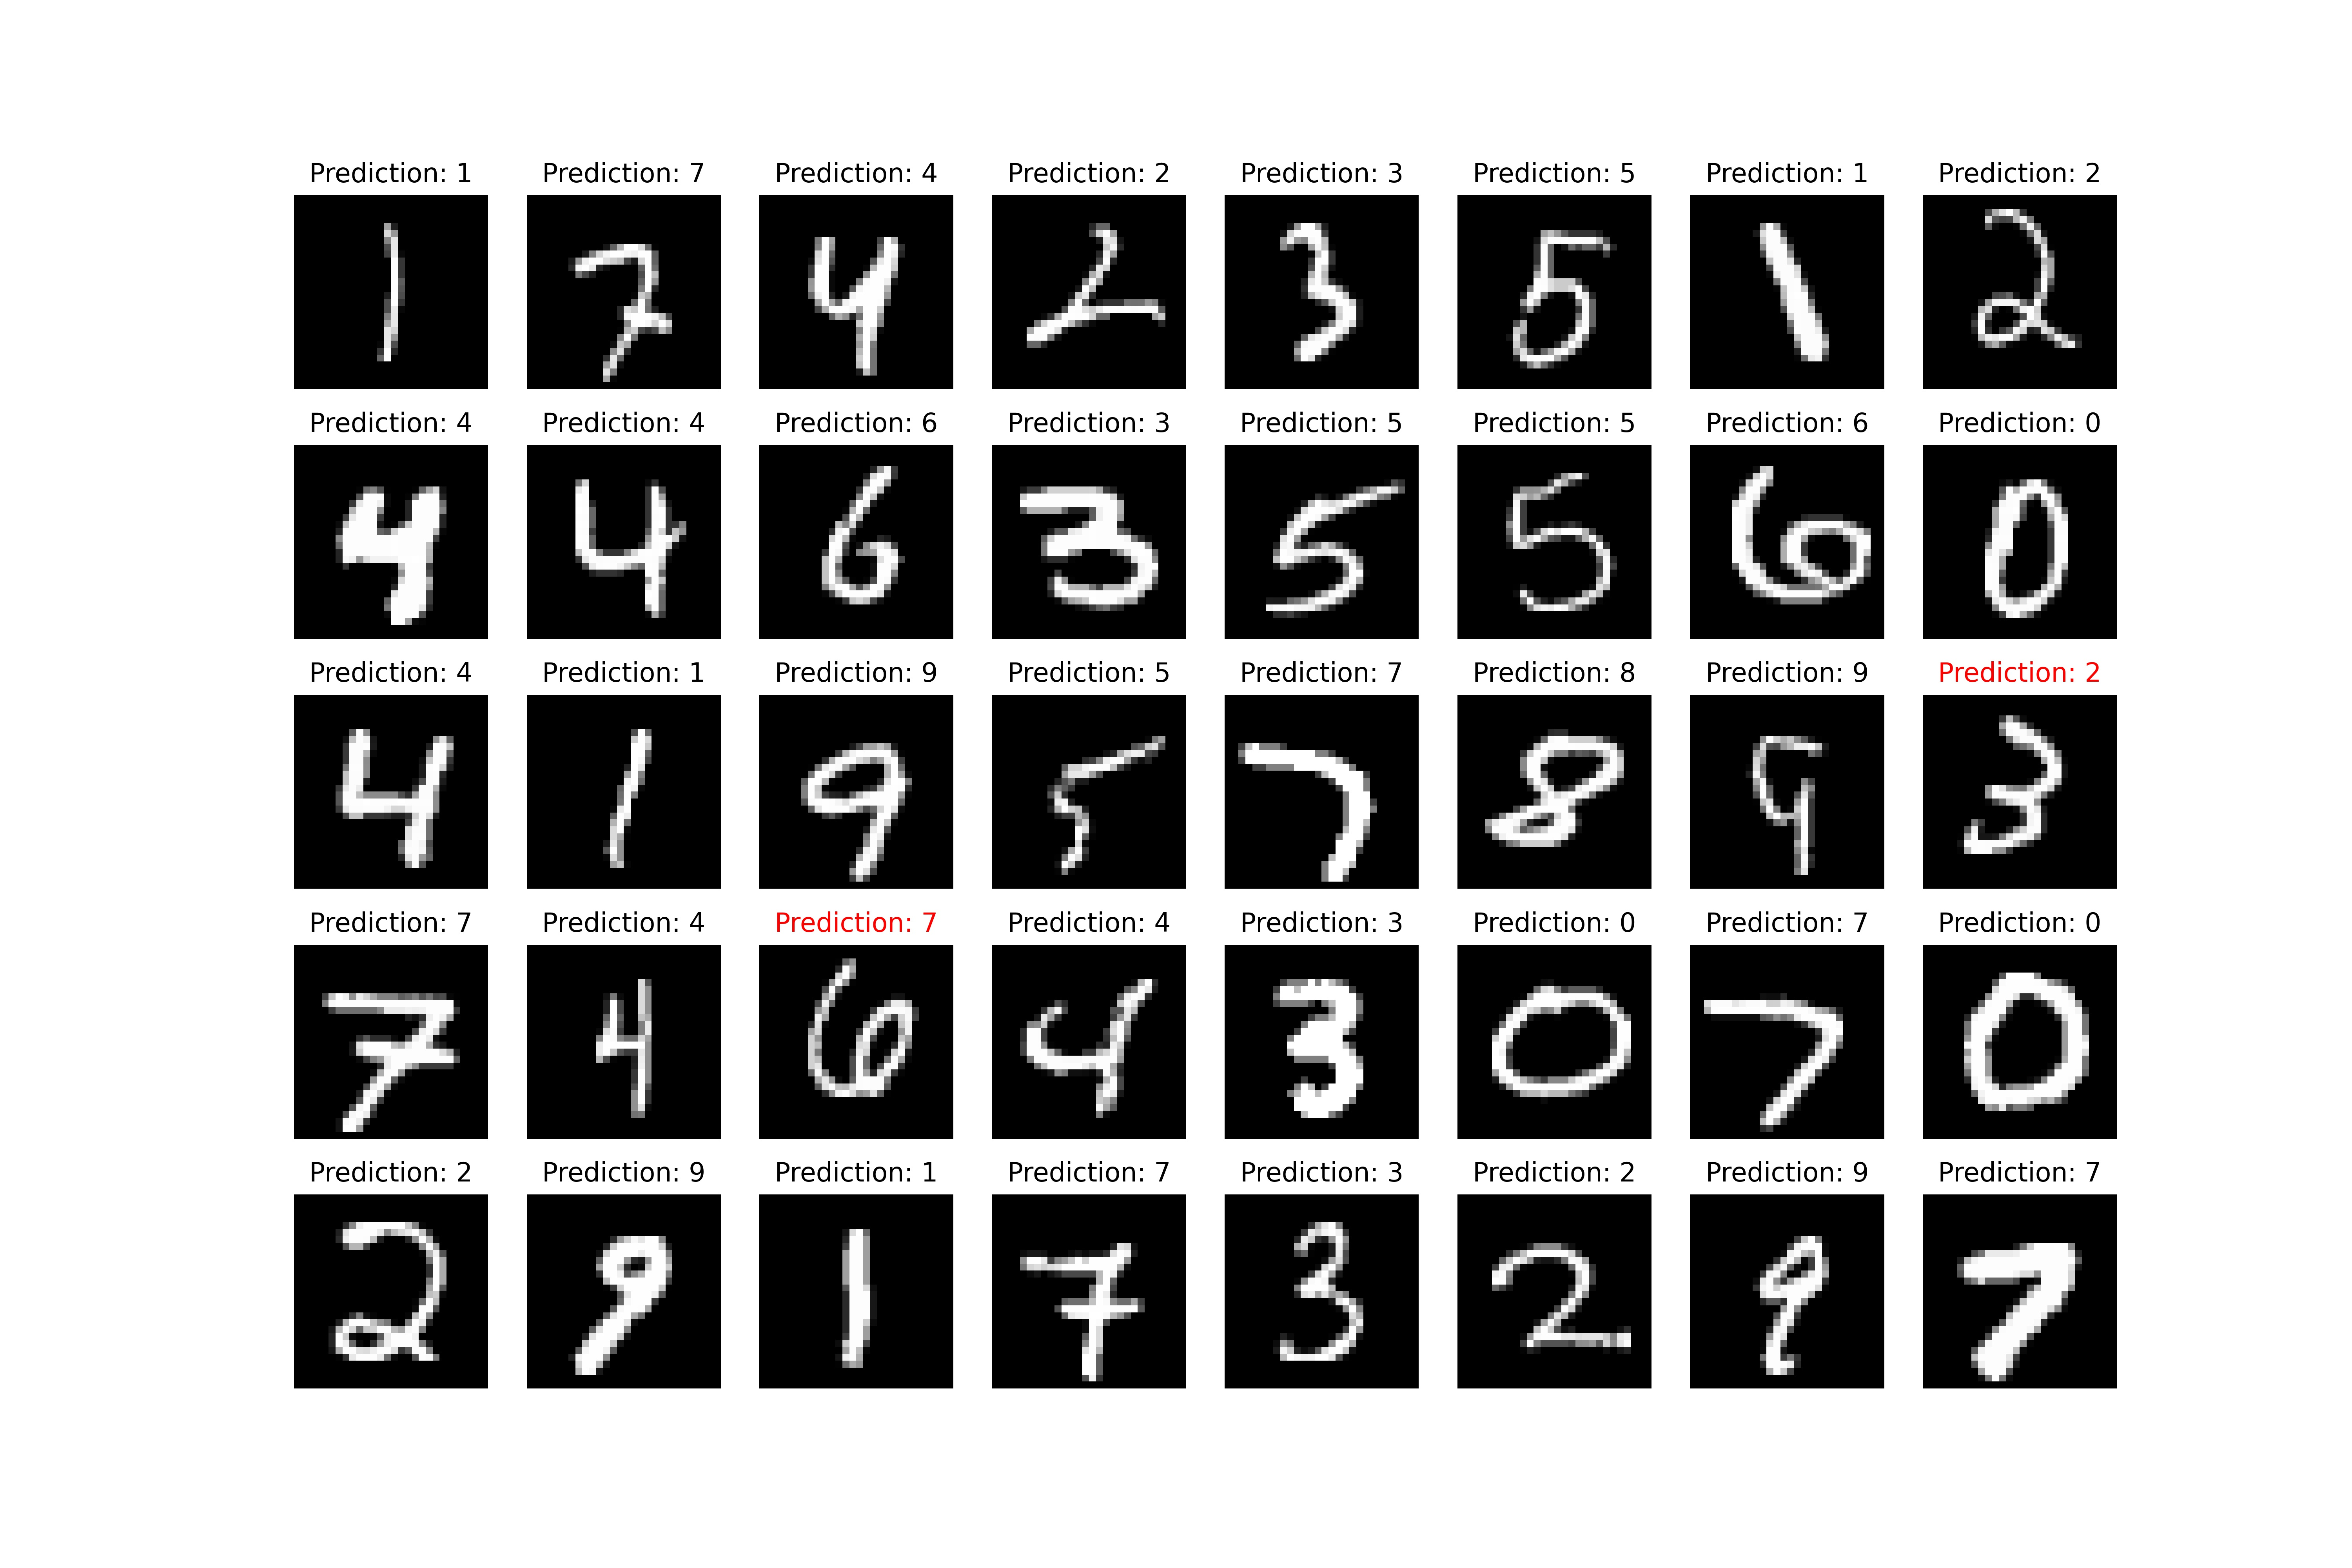
\includegraphics[height=170px]{4-Resultat.jpg}
		\caption{Exemple sur un échantillon de 40 images de validation}
	\end{figure}
\end{frame}


% 3-3 Reconnaissance d’image de vêtements 
\subsection{Convolution d'image}



\begin{frame}{Une base de données plus complexe}
    \begin{block}{Deux façons différentes de faire du traitement d'image}
        \begin{itemize}
            \item L'image $28\times28$ pixels est aplatie en un vecteur de taille $784$.
            \item L'image 2D est directement prise en entrée du réseau de neurones.
        \end{itemize}
    \end{block}
    \begin{columns}
        \begin{column}{0.5\textwidth}
            \begin{figure}
                \centering
                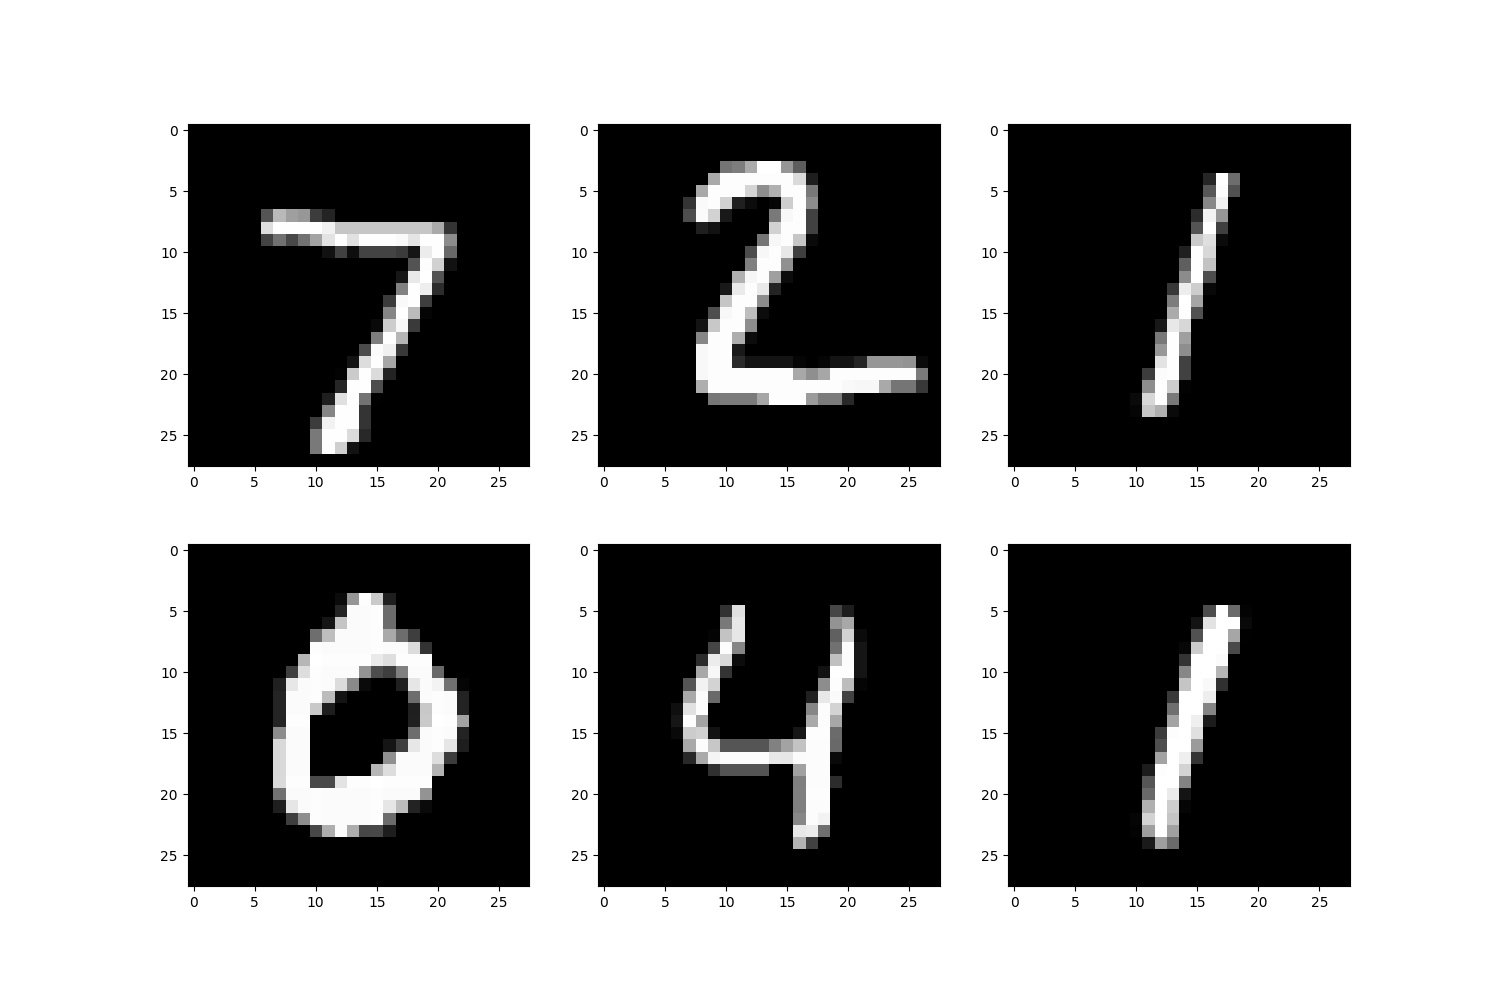
\includegraphics[width=\textwidth]{1-mnist.jpg}
                \caption{Chiffres écrits à la main}
            \end{figure}
        \end{column}
        \begin{column}{0.5\textwidth}
            \begin{figure}
                \centering
                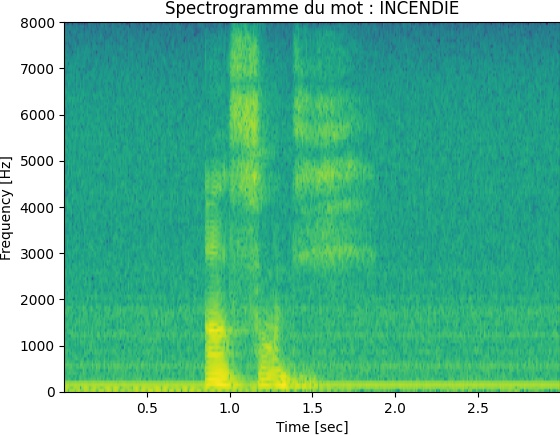
\includegraphics[width=0.9\textwidth]{1-Incendie.jpg}
                \caption{Spectrogramme}
            \end{figure}
        \end{column}
    \end{columns}
\end{frame}

\begin{frame}{La convolution d'image}
    \begin{figure}
        \centering
        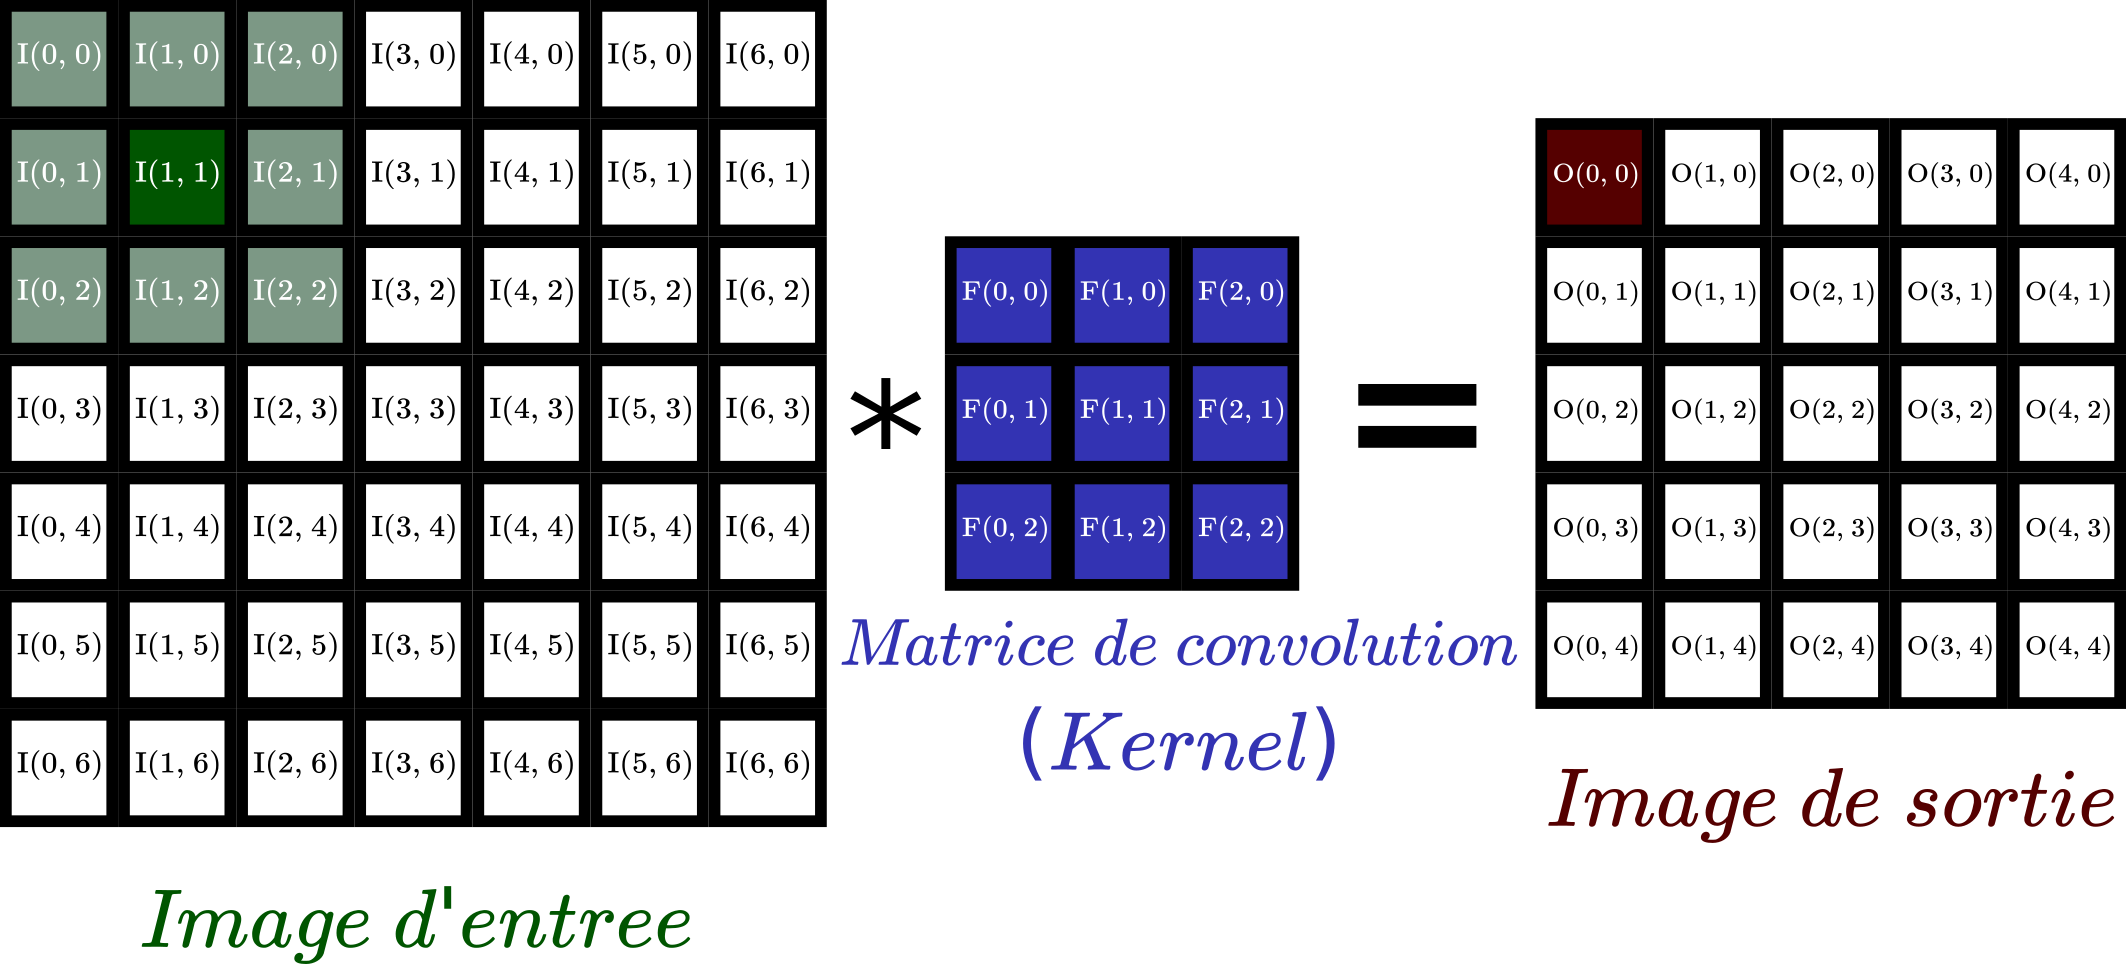
\includegraphics[width=\textwidth]{5-convolution.png}
        \centering
        \caption{Schéma de la convolution d'image $O(0, 0) = \sum_{i=0}^{2}\sum_{j=0}^{2}I(i, j)\times F(i, j)$}
    \end{figure}
\end{frame}


\begin{frame}{Un exemple de convolution d'image}
    \begin{columns}[T] % align columns
        \begin{column}{.6\textwidth}
            \begin{figure}
                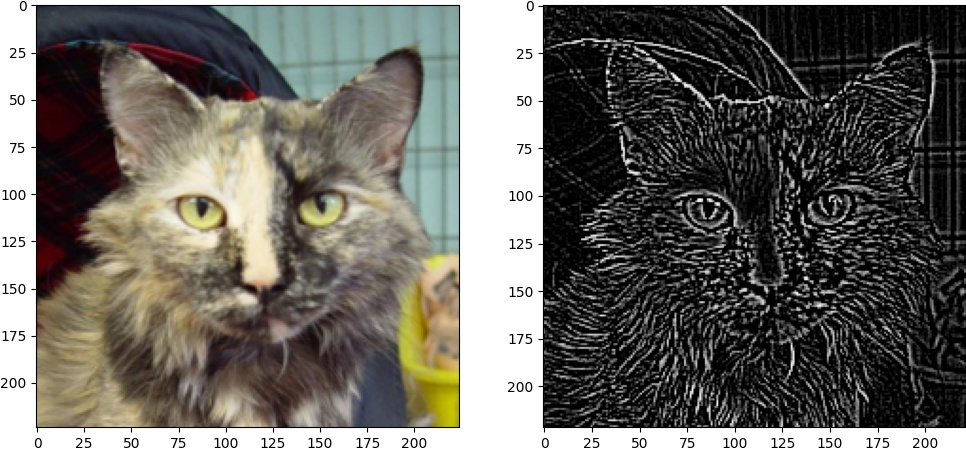
\includegraphics[width=\textwidth]{6-cat.jpg}
                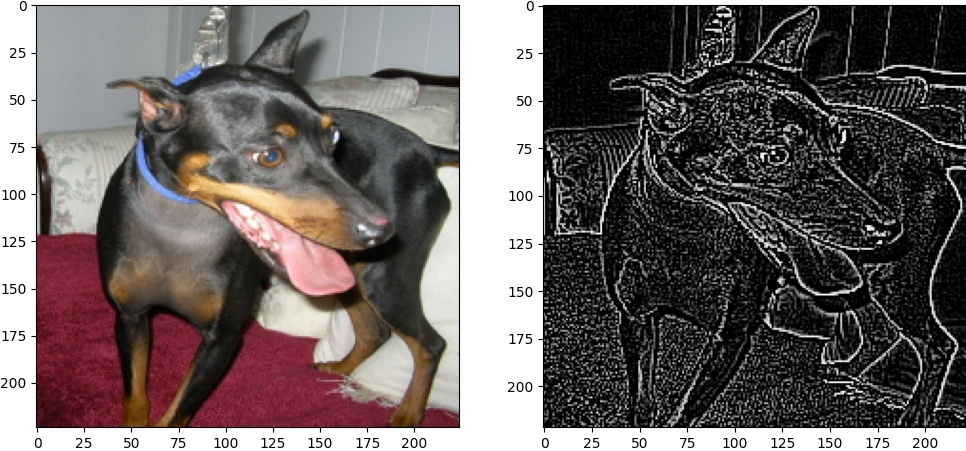
\includegraphics[width=\textwidth]{6-dog.jpg}
                \caption[]{Exemple de convolution d'image}
            \end{figure}
        \end{column}
        \begin{column}{0.35\textwidth}
            \begin{exampleblock}{Détection de contour}
                \begin{center}
                    \centering
                    $
                        F =
                        \begin{pmatrix}
                            -1 & -1 & -1 \\
                            -1 & 8  & -1 \\
                            -1 & -1 & -1
                        \end{pmatrix}
                    $
                \end{center}
            \end{exampleblock}
        \end{column}
    \end{columns}
\end{frame}


\begin{frame}{Le schéma du réseau de neurones convolutif}
    \begin{figure}
        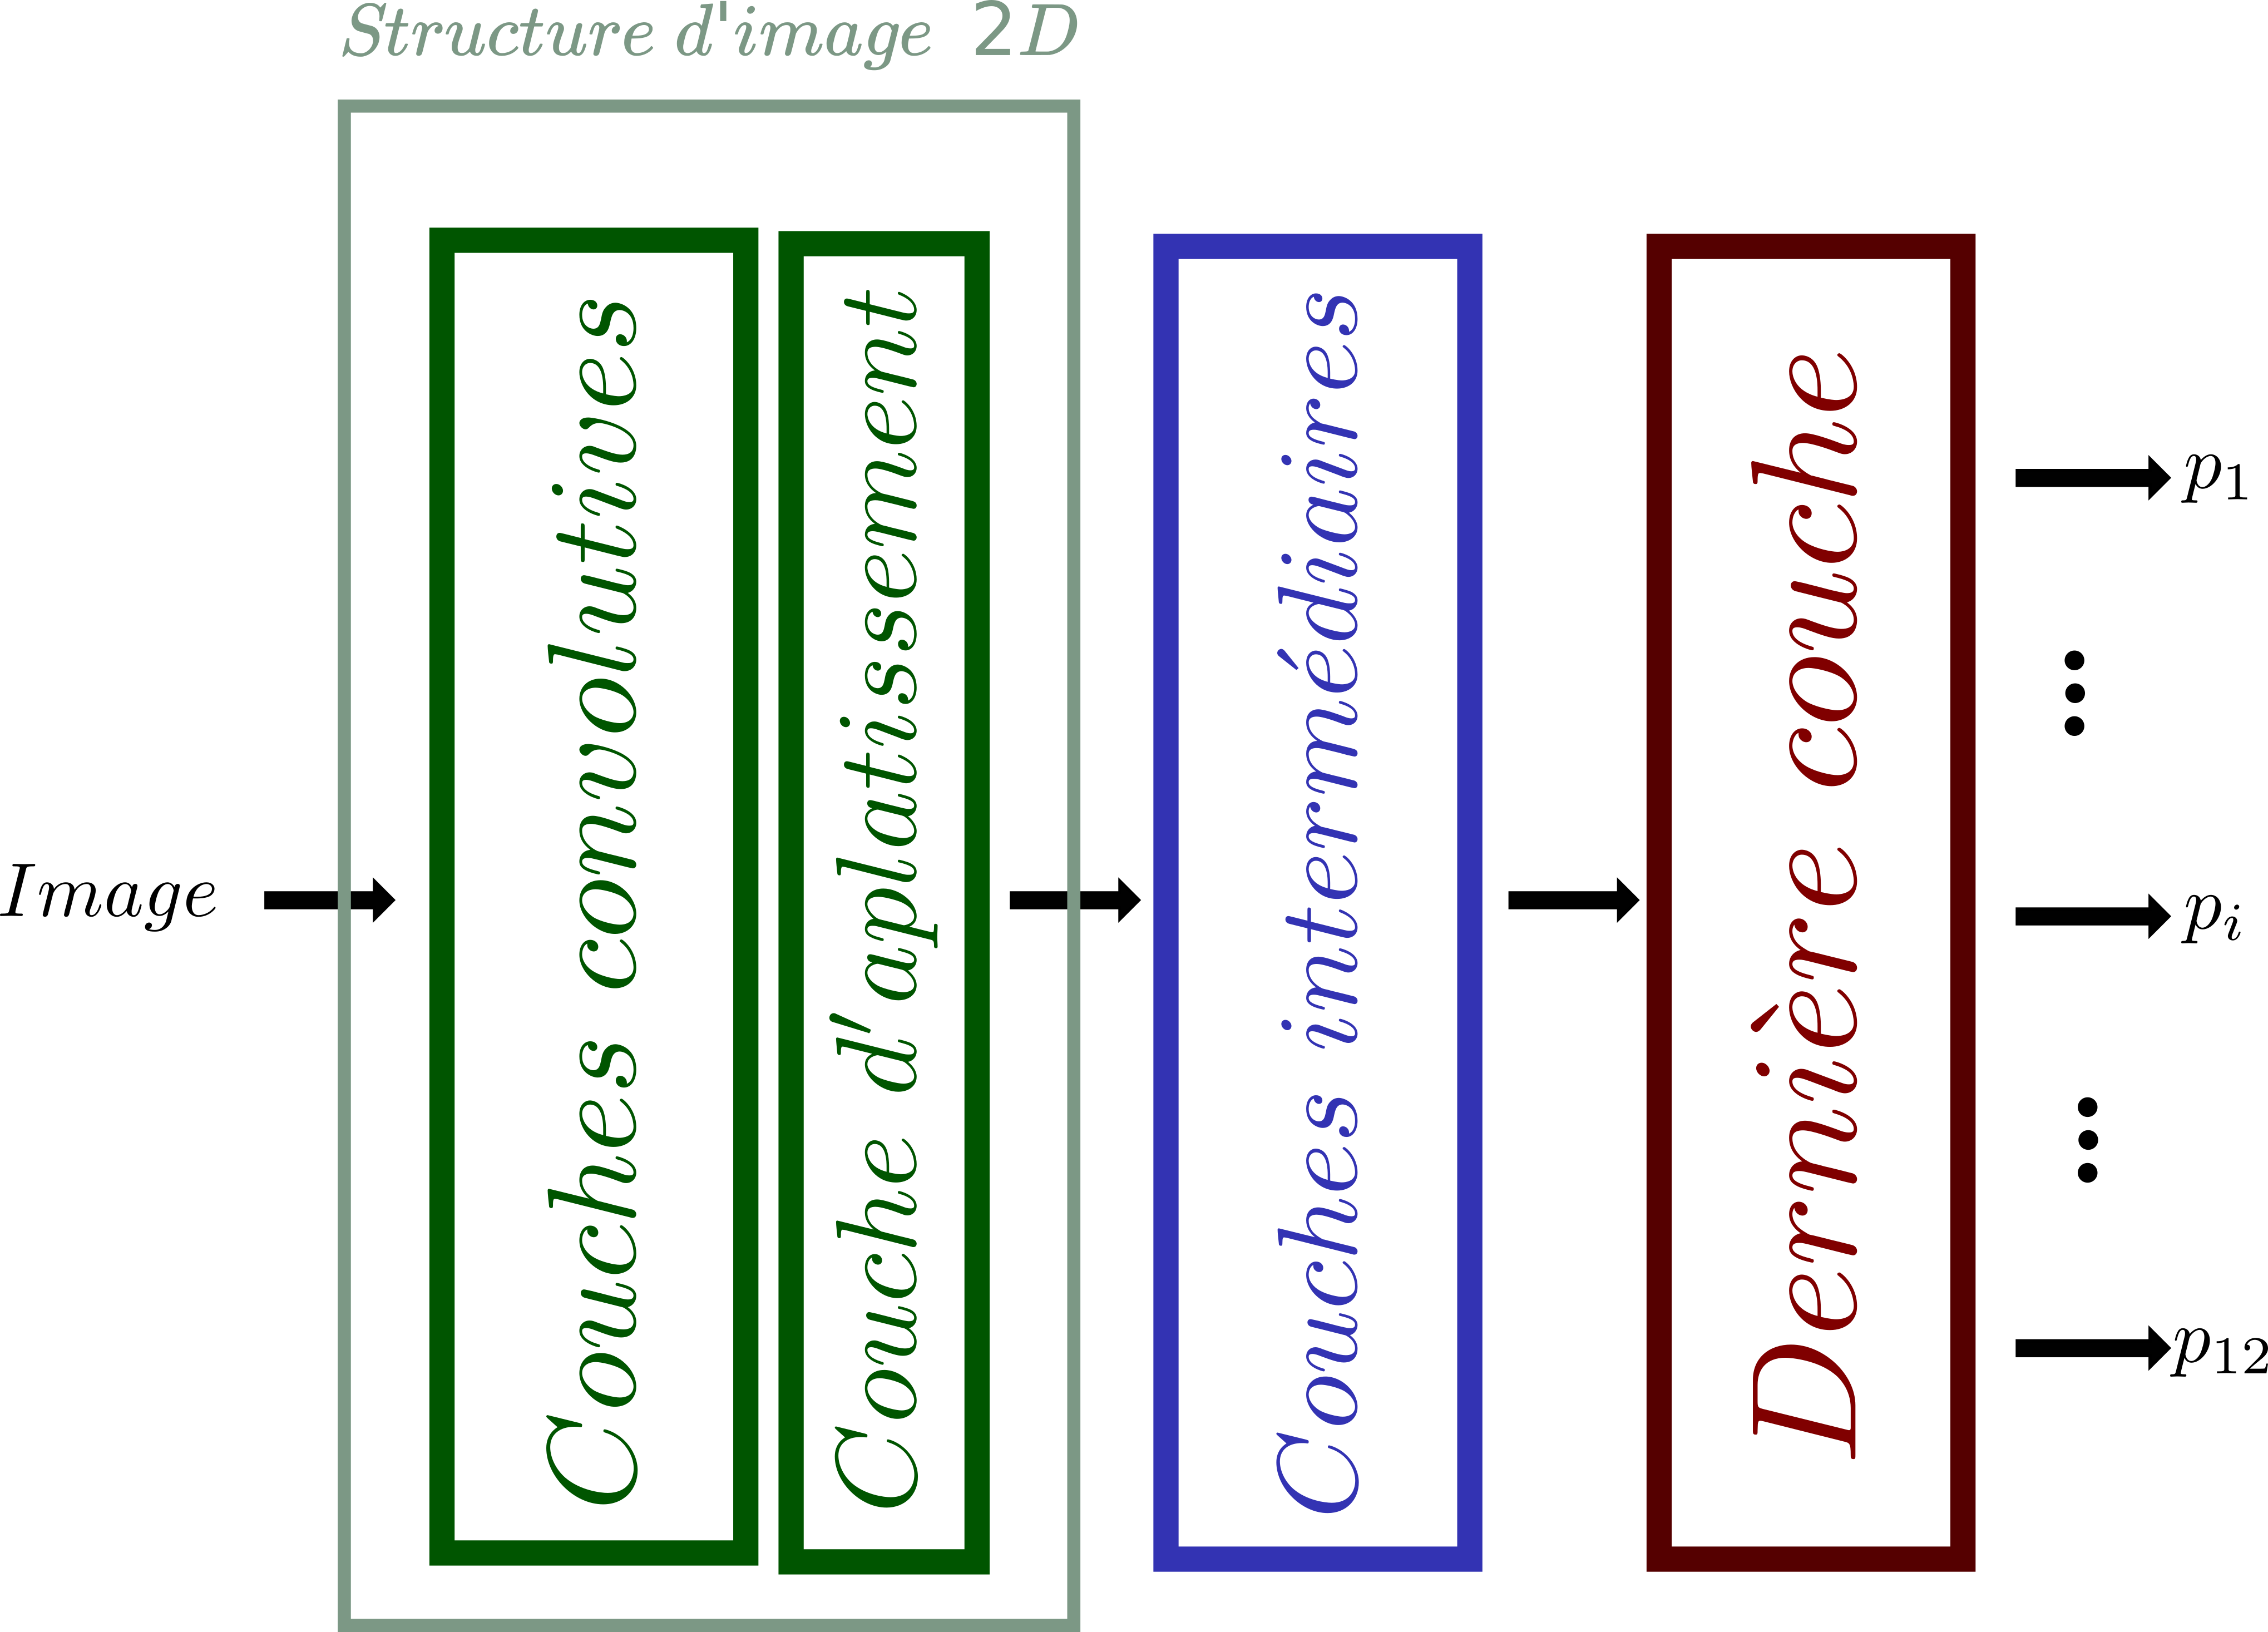
\includegraphics[height=0.7\textheight]{9-reseau convolutif.png}
        \caption[]{Schéma de réseau de neurones convolutif}
    \end{figure}
\end{frame}

% 3-4 Reconnaissance vocale de mots-clés
\subsection{Reconnaissance vocale de mots-clés}


\begin{frame}{La reconnaissance de mots-clés}
	\begin{block}{}
		\begin{description}
			\item[n°15] malaise, hémorragie, brûlure, intoxication
			\item[n°17] violences, agression, vol, cambriolage
			\item[n°18] incendie, gaz, effondrement, électrocution
		\end{description}
	\end{block}
	\begin{figure}
		\begin{subfigure}[]{0.31\textwidth}
			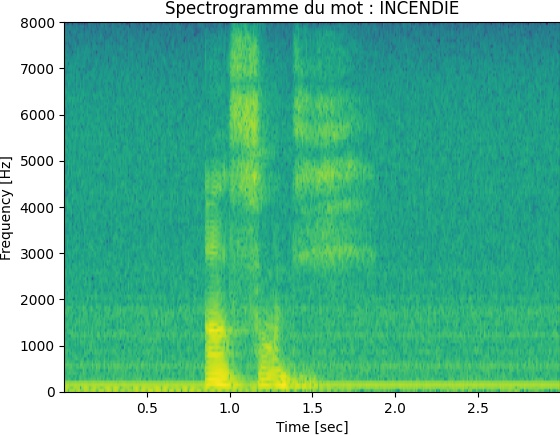
\includegraphics[width=\textwidth]{1-Incendie.jpg}
			\caption{INCENDIE}
		\end{subfigure}
		\begin{subfigure}[]{0.31\textwidth}
			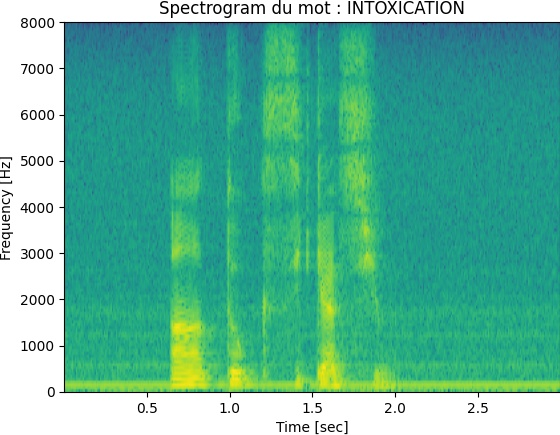
\includegraphics[width=\textwidth]{1-Intoxication.jpg}
			\caption{INTOXICATION}
		\end{subfigure}
		\begin{subfigure}[]{0.31\textwidth}
			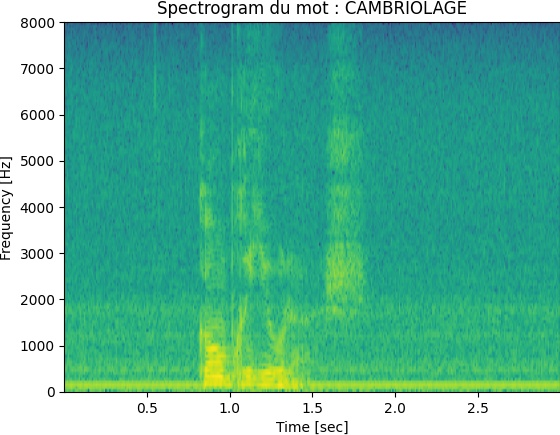
\includegraphics[width=\textwidth]{1-Cambriolage.jpg}
			\caption{CAMBRIOLAGE}
		\end{subfigure}
	\end{figure}
\end{frame}


\begin{frame}{La création de la base de données}
	\begin{columns}[T]
		\begin{column}[]{0.45\textwidth}
			\begin{exampleblock}{Données d'apprentissage}
				\begin{description}
					\item[Agathe]  $1\times12$ données
					\item[Florent]  $1\times12$ données
					\item[Tien-Thinh]  $4\times12$ données
				\end{description}
			\end{exampleblock}
		\end{column}
		\begin{column}[]{0.45\textwidth}
			\begin{alertblock}{Données d'évaluation}
				\begin{description}
					\item[Agathe]  $1\times12$ données
					\item[Florent]  $1\times12$ données
					\item[Tien-Thinh]  $1\times12$ données
				\end{description}
			\end{alertblock}
		\end{column}
	\end{columns}
	\begin{block}{Problématiques}
		\begin{itemize}
			\item Les spectrogrammes sont trop grands de tailles 374*129
			\item Trop peu de données pour la rétropropagation
		\end{itemize}
	\end{block}
\end{frame}




\begin{frame}{Le transfert d'apprentissage à partir d'un réseau modèle}
	\begin{block}{Le réseau de neurones modèle}
		Il est entrainé sur 8 000 données pour reconnaitre les $8$ mots : \\
		$["no",\ "stop",\ "up",\ "right",\ "yes",\ "left",\ "go",\ "down"]$ \\
	\end{block}
	\begin{exampleblock}{L'adaptation}
		\begin{itemize}
			\item La durée des audios est différente
			\item Le nombre de sortie est différent
		\end{itemize}
	\end{exampleblock}
\end{frame}



\begin{frame}{Un schéma du transfert d'apprentissage}
	\begin{figure}
		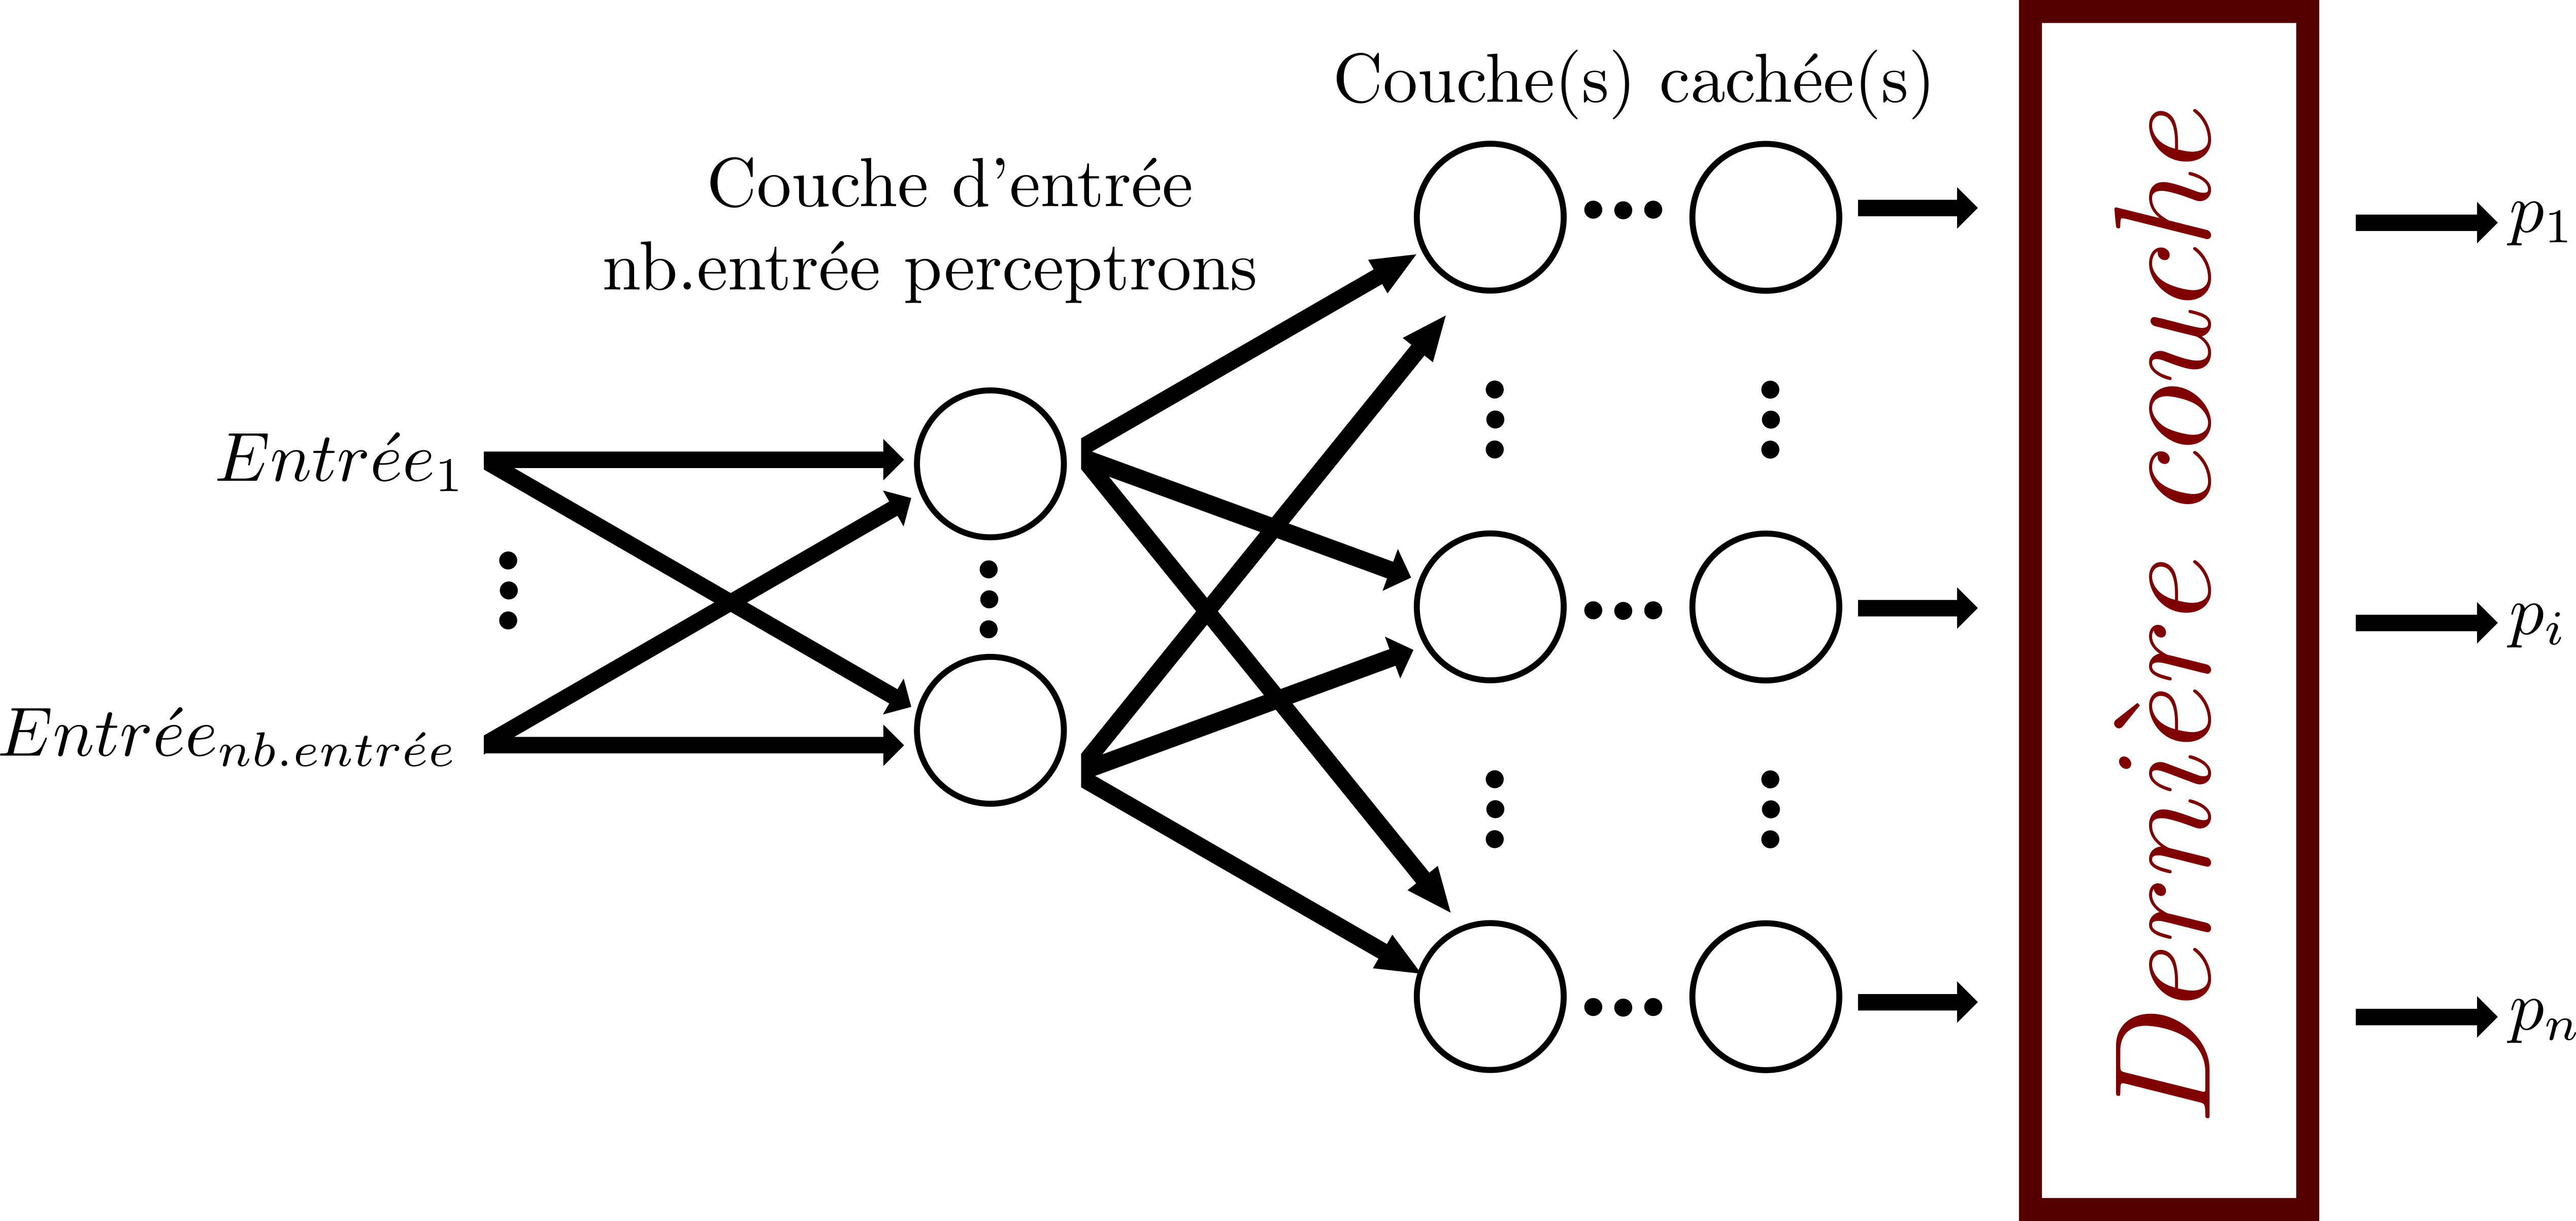
\includegraphics[width=\textwidth]{2-transfert.png}
		\caption{Schéma de fonctionnement du transfert d'apprentissage}
	\end{figure}
\end{frame}


\begin{frame}{Mes résultats}
	\begin{figure}
		\begin{subfigure}[]{0.49\textwidth}
			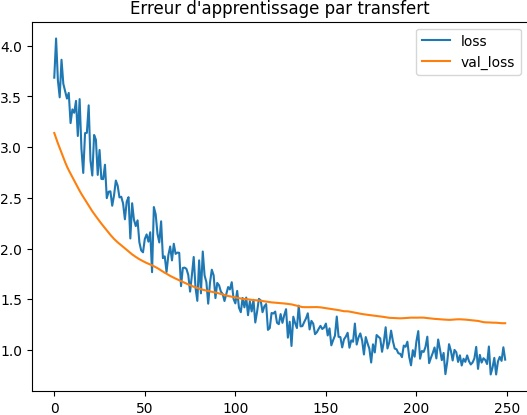
\includegraphics[width=\textwidth]{4-loss.jpg}
			\caption{Erreur au cours de l'apprentissage}
		\end{subfigure}
		\begin{subfigure}[]{0.49\textwidth}
			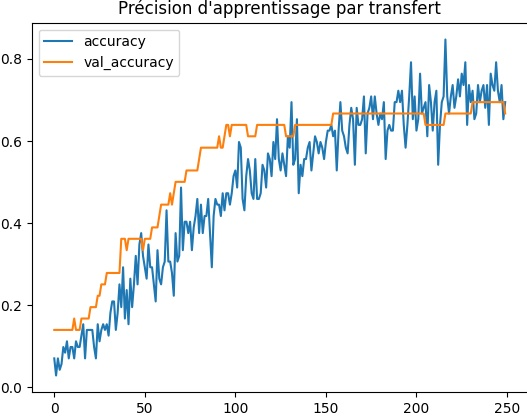
\includegraphics[width=\textwidth]{4-accuracy.jpg}
			\caption{Taux de bonnes réponses}
		\end{subfigure}
	\end{figure}
	\begin{columns}[T]
		\begin{column}{0.25\textwidth}
		\end{column}
		\begin{column}[]{0.50\textwidth}
			\begin{block}{Précision finale}
				\begin{description}
					\item[Agathe]  $50\%$ accuracy
					\item[Florent]  $75\%$ accuracy
					\item[Tien-Thinh]  $75\%$ accuracy
				\end{description}
			\end{block}
		\end{column}
		\begin{column}{0.25\textwidth}
		\end{column}
	\end{columns}
\end{frame}



\begin{frame}{Conclusion : Schéma de la réalisation du réseau de neurones}
	\begin{figure}
		\centering
		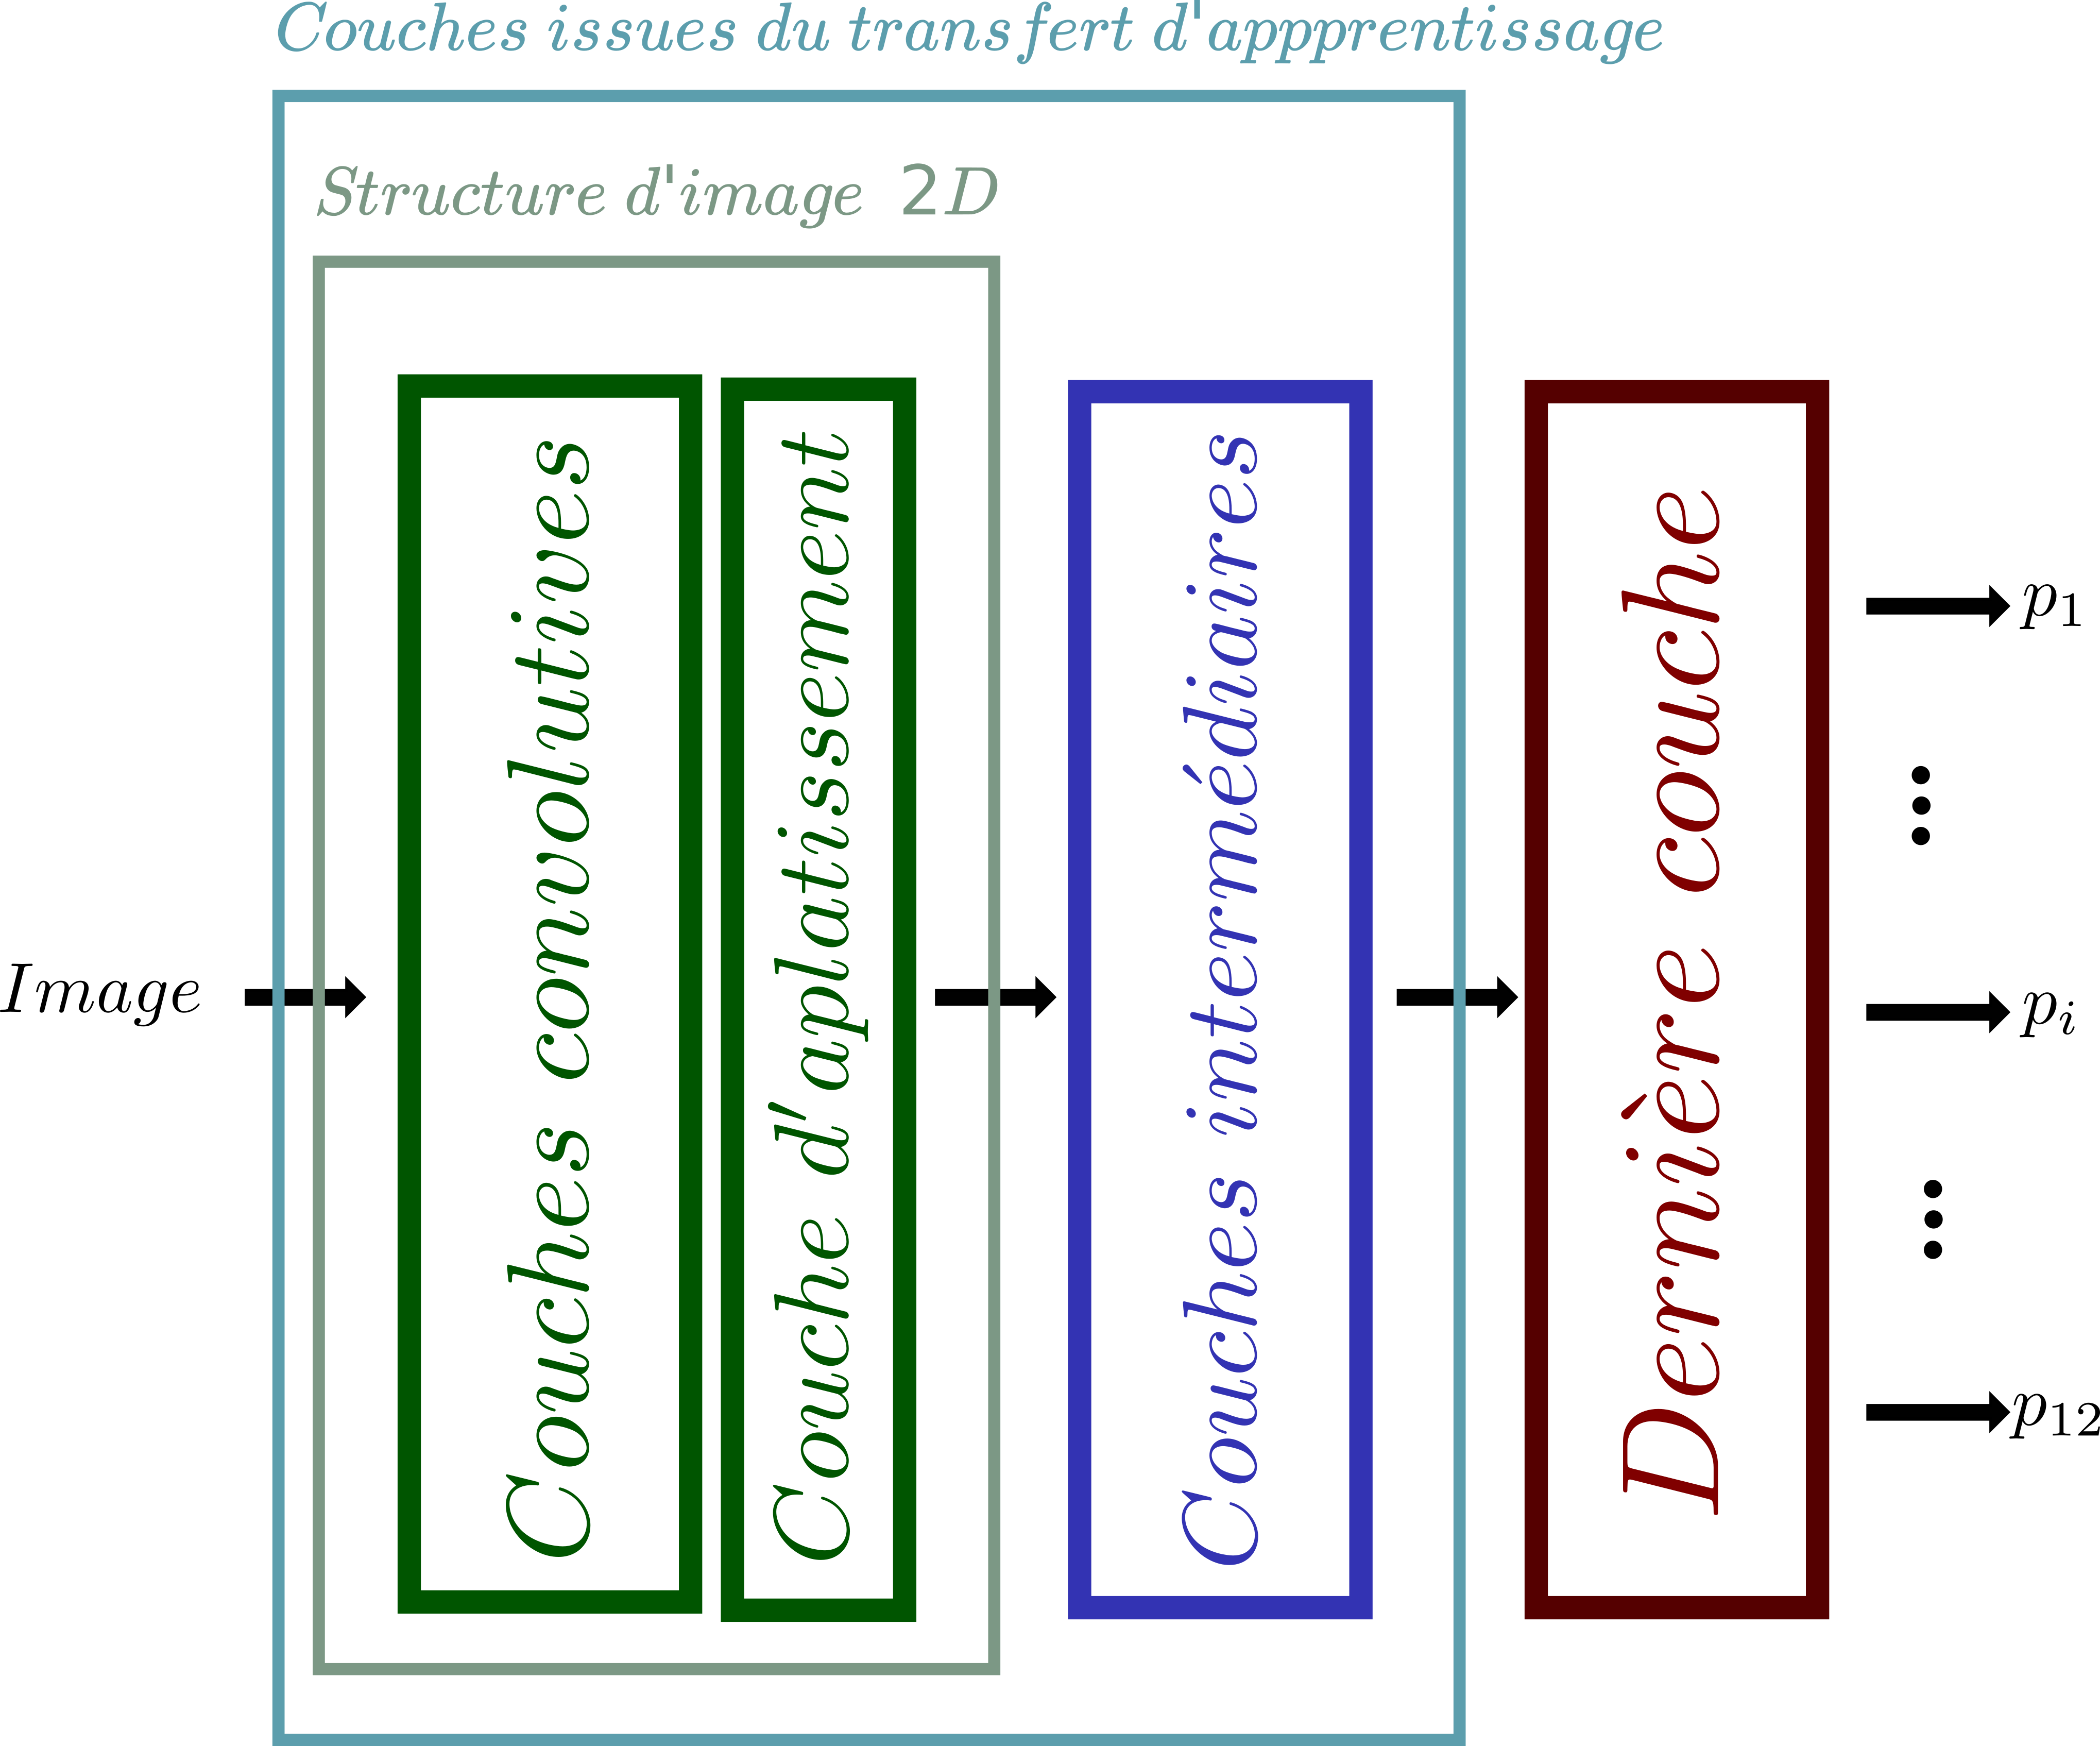
\includegraphics[height=0.7\textheight]{6-schema.png}
		\caption{Structure de mon réseau de neurones}
	\end{figure}
\end{frame}


\begin{frame}{Conclusion : Les moteurs de reconnaissance vocale}
	\begin{figure}
		\begin{center}
			\centering
			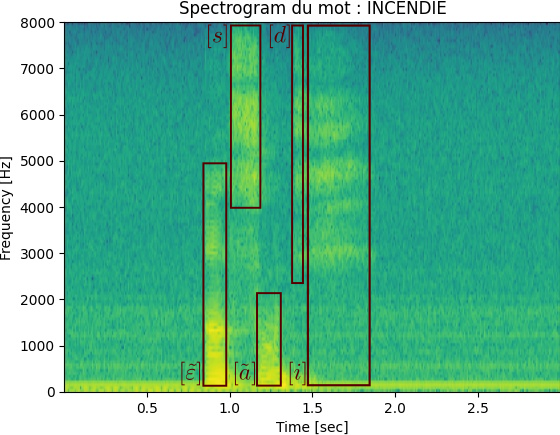
\includegraphics[width=0.4\textwidth]{3-incendie.png}
			\caption{Analyse du mot "INCENDIE"}
		\end{center}
	\end{figure}

	\begin{exampleblock}{Les performances moyennes des moteurs de reconnaissance vocale}
		\begin{itemize}
			\item Textes lus (dictée vocale, système monolocuteur) : 95 \%
			\item Journaux radio et TV : 90 \%
			\item Conversations téléphoniques informelles : 60 \%
		\end{itemize}
	\end{exampleblock}
\end{frame}




% 4 Annexe
\section{Annexe}
% 4-1 Mes codes
\subsection{Mes classes}


\begin{frame}{Annexe}
    \lstinputlisting[language=Python]{requirements.py}
\end{frame}


\begin{frame}[fragile, allowframebreaks]{NeuroneLineaire.py}
    \lstinputlisting[language=Python, firstline=15]{NeuroneLineaire.py}
\end{frame}


\begin{frame}[fragile]{Activation.py}
    \lstinputlisting[language=Python, firstline=15, basicstyle=\ttfamily\tiny]{Activation.py}
\end{frame}


\begin{frame}[fragile]{Loss.py}
    \lstinputlisting[language=Python, firstline=15]{Loss.py}
\end{frame}


\begin{frame}[fragile, allowframebreaks]{Layer.py}
    \lstinputlisting[language=Python, firstline=15]{Layer.py}
\end{frame}


\begin{frame}[fragile, allowframebreaks]{Convolutional.py}
    \lstinputlisting[language=Python, firstline=15]{Convolutional.py}

\end{frame}


\begin{frame}[fragile, allowframebreaks]{Model.py}
    \lstinputlisting[language=Python, firstline=15]{Model.py}
\end{frame}


\begin{frame}[fragile]{AugmentationDonnee.py}
    \lstinputlisting[language=Python, firstline=15, basicstyle=\ttfamily\tiny]{Augmentation_Donnee.py}
\end{frame}




\end{document}